% !TEX program = xelatex
\documentclass[12pt,a4paper]{report}
\usepackage{fontspec}   % XeLaTeX: native Unicode (Vietnamese) rendering
\usepackage{lmodern}
\usepackage{amsmath,amssymb}
\usepackage{graphicx}
\graphicspath{{figures/}{./}{../figures/}}
\usepackage{booktabs,longtable,array,calc}
\usepackage{caption}
\usepackage{float}
\usepackage{microtype}
\usepackage[a4paper,top=2cm,bottom=2cm,left=2.5cm,right=2.5cm]{geometry}
\usepackage{tikz}
\usetikzlibrary{arrows.meta}
\usepackage{xcolor}
\usepackage[hidelinks]{hyperref}
\usepackage{parskip}
\usepackage{textcomp}
\usepackage{newunicodechar}
\newunicodechar{§}{\S}
\newunicodechar{·}{\textperiodcentered}
\newunicodechar{…}{\ldots}
\newunicodechar{–}{--}
\newunicodechar{—}{---}
\newunicodechar{°}{\textdegree}
\newunicodechar{±}{\ensuremath{\pm}}
\newunicodechar{×}{\ensuremath{\times}}
\newunicodechar{≈}{\ensuremath{\approx}}
\newunicodechar{≠}{\ensuremath{\neq}}
\newunicodechar{≥}{\ensuremath{\geq}}
\newunicodechar{≤}{\ensuremath{\leq}}
\newunicodechar{→}{\ensuremath{\rightarrow}}
\newunicodechar{←}{\ensuremath{\leftarrow}}
\newunicodechar{−}{\ensuremath{-}}
\newunicodechar{∇}{\ensuremath{\nabla}}
\newunicodechar{∅}{\ensuremath{\emptyset}}
\newunicodechar{△}{\ensuremath{\triangle}}
\newunicodechar{θ}{\ensuremath{\theta}}
\newunicodechar{π}{\ensuremath{\pi}}
\newunicodechar{α}{\ensuremath{\alpha}}
\newunicodechar{†}{\textdagger}
\newunicodechar{⚠}{\textbf{!}}

\usepackage{listings}
\lstset{basicstyle=\ttfamily\footnotesize,breaklines=true,breakatwhitespace=false,
  columns=fullflexible,keepspaces=true,showstringspaces=false,frame=none,
  breakindent=0pt,postbreak=\mbox{\textcolor{gray}{$\hookrightarrow$}\space}}
\usepackage{etoolbox}
\AtBeginEnvironment{longtable}{\small}
\AtBeginEnvironment{verbatim}{\footnotesize}

\providecommand{\tightlist}{\setlength{\itemsep}{0pt}\setlength{\parskip}{0pt}}
\providecommand{\passthrough}[1]{#1}
\providecommand{\pandocbounded}[1]{#1}
\providecommand{\real}[1]{#1}

\setcounter{secnumdepth}{3}
\setcounter{tocdepth}{2}

% ---- Vietnamese caption / label names ----
\renewcommand{\chaptername}{Chương}
\renewcommand{\contentsname}{Mục lục}
\renewcommand{\listfigurename}{Danh sách hình vẽ}
\renewcommand{\listtablename}{Danh sách bảng}
\renewcommand{\bibname}{Tài liệu tham khảo}
\renewcommand{\figurename}{Hình}
\renewcommand{\tablename}{Bảng}
\renewcommand{\appendixname}{Phụ lục}

% compact chapter headings
\usepackage{titlesec}
\titleformat{\chapter}[display]{\normalfont\bfseries\Huge}{\chaptertitlename\ \thechapter}{6pt}{\Huge}
\titlespacing*{\chapter}{0pt}{4pt}{16pt}

\begin{document}

% ============================ OUTER COVER ============================
\begin{titlepage}
\centering
{\normalsize\bfseries ĐẠI HỌC QUỐC GIA TP. HỒ CHÍ MINH\par}
{\normalsize\bfseries TRƯỜNG ĐẠI HỌC KHOA HỌC TỰ NHIÊN\par}
\vspace{1.2cm}

\includegraphics[width=3.4cm]{../figures/khtn_logo.png}\par
\vspace{1.8cm}
{\large\bfseries Mai Phong Đăng\par}
\vspace{1.6cm}
{\Large\bfseries TĂNG TỐC KHÁM PHÁ LỜI GIẢI TẠI THỜI ĐIỂM SUY LUẬN TRONG BÀI TOÁN SINH MÃ PHỨC TẠP BẰNG PHƯƠNG PHÁP TỰ CHƯNG CẤT DỰA TRÊN PHẢN HỒI THỰC THI\par}
\vspace{1.3cm}
{\large\bfseries KHÓA LUẬN TỐT NGHIỆP ĐẠI HỌC\par}
\vfill
{\normalsize Thành phố Hồ Chí Minh, tháng 7 năm 2026\par}
\end{titlepage}

% ============================ INNER COVER ============================
\begin{titlepage}
\centering
{\normalsize\bfseries TRƯỜNG ĐẠI HỌC KHOA HỌC TỰ NHIÊN, ĐHQG-HCM\par}
{\normalsize\bfseries Khoa Toán -- Tin học\par}
{\normalsize\bfseries Ngành Khoa học Dữ liệu\par}
\vspace{2.2cm}
{\large\bfseries Mai Phong Đăng \hspace{2em} 22280008\par}
\vspace{1.8cm}
{\Large\bfseries TĂNG TỐC KHÁM PHÁ LỜI GIẢI TẠI THỜI ĐIỂM SUY LUẬN TRONG BÀI TOÁN SINH MÃ PHỨC TẠP BẰNG PHƯƠNG PHÁP TỰ CHƯNG CẤT DỰA TRÊN PHẢN HỒI THỰC THI\par}
\vspace{1.3cm}
{\large\bfseries KHÓA LUẬN TỐT NGHIỆP ĐẠI HỌC\par}
\vspace{2.0cm}
{\large\bfseries Giảng viên hướng dẫn: TS. Ngô Minh Mẫn\par}
\vfill
{\normalsize Thành phố Hồ Chí Minh, tháng 7 năm 2026\par}
\end{titlepage}

\chapter*{Tóm tắt}
\addcontentsline{toc}{chapter}{Tóm tắt}
Test-time training cho một mô hình ngôn ngữ khả năng tự cải thiện ngay tại
thời điểm suy luận, trên một bài toán khó duy nhất. Nhưng self-distillation
theo kiểu on-policy rất dễ giậm chân tại chỗ: nếu mô hình không thể tự sinh
ra một lời giải đúng, thì cũng chẳng có gì đúng để nó học theo. Khóa luận
này tìm cách tăng tốc test-time discovery trong sinh mã phức tạp bằng
\emph{execution-guided self-distillation}: dùng execution feedback
(test case thất bại, lỗi runtime) làm privileged context dẫn dắt từng
bước cập nhật. Tôi đề xuất một cách tổ chức \emph{teacher-first}:
thay vì distill chính rollout thất bại của student, self-teacher sinh
trước các quỹ đạo dưới feedback; một verifier và một judge lọc chúng theo
tính đúng và tính độc lập; rồi student mới được distill về phía những quỹ
đạo đã qua lọc đó. Cách tổ chức này đặt phương pháp đề xuất ở vị trí giao
thoa giữa SDPO on-policy và SFT off-policy. Trong một đánh giá đối chiếu
(matched evaluation) quy mô trung bình trên các bài toán LiveCodeBench khó
bằng mô hình 4B, teacher-first vượt trội đáng kể so với baseline
student-first (kiểm định Wilcoxon signed-rank). Đặc biệt trên những bài khó
nhất, phương pháp này thoát được flat-reward trap, cạm bẫy vốn luôn
khiến student-first giậm chân tại mức 0. Một so sánh cân bằng tính toán
(compute-matched) cho thấy lợi thế này không phải là hệ quả ảo sinh ra từ
khối lượng lấy mẫu: ở cùng một ngân sách generation, teacher-first vẫn
chiến thắng và đạt được xác suất khám phá (discovery) mục tiêu với số
lượng generation ít hơn đáng kể. Khi kích hoạt cơ chế suy nghĩ (thinking),
tôi tiến hành đo lường epistemic verbalization tại thời điểm suy luận và
phát hiện ra rằng: quá trình chưng cất (distill) từ một feedback-conditioned
context làm suy giảm các uncertainty marker, một minh chứng trực tiếp
cho hiện tượng suy giảm mà Kim và cộng sự đã mô tả. Cuối cùng, việc đánh
giá pipeline trên tác vụ suy luận toán học (AIME 2026) đã vạch rõ một ranh
giới áp dụng rất nghiêm ngặt (rigid domain boundary): khi feedback chỉ gói
gọn trong một giá trị số tĩnh thay vì một quy trình thuật toán, teacher
policy sẽ suy biến thành hành vi sao chép đáp án nông cạn mà không mang
lại bất kỳ sự cải thiện năng lực nào, qua đó thiết lập nên một ràng buộc
khắt khe giữa quy trình và giá trị (procedure-versus-value) đối với
self-distillation tại thời điểm suy luận.

\vspace{0.5cm}
\textbf{Từ khóa:} test-time training, self-distillation, sinh mã,
execution feedback, discovery@k, epistemic suppression, ranh giới miền.


\tableofcontents

\clearpage
\addcontentsline{toc}{chapter}{Danh sách hình vẽ}
\listoffigures

\clearpage
\addcontentsline{toc}{chapter}{Danh sách bảng}
\listoftables

\clearpage
\chapter*{Danh sách từ viết tắt}
\addcontentsline{toc}{chapter}{Danh sách từ viết tắt}
\begin{longtable}{@{}p{2.6cm}l@{}}
AIME & American Invitational Mathematics Examination \\
EMA  & Exponential Moving Average \\
GRPO & Group Relative Policy Optimization \\
JSD  & Jensen--Shannon Divergence \\
KL   & Kullback--Leibler (divergence) \\
LCB  & LiveCodeBench \\
LLM  & Large Language Model (mô hình ngôn ngữ lớn) \\
LoRA & Low-Rank Adaptation \\
PPO  & Proximal Policy Optimization \\
RLRF & Reinforcement Learning with Rich Feedback \\
RLVR & Reinforcement Learning with Verifiable Rewards \\
RO   & Research Objective (mục tiêu nghiên cứu) \\
SDFT & Self-Distillation Fine-Tuning \\
SDPO & Self-Distillation Policy Optimization \\
SF   & Student-First \\
SFT  & Supervised Fine-Tuning \\
TF   & Teacher-First \\
TRL  & Transformer Reinforcement Learning (thư viện) \\
TTT  & Test-Time Training \\
\end{longtable}

\chapter{Giới thiệu}\label{chapter-1-introduction}

Khóa luận này nghiên cứu cách tăng tốc test-time discovery trong sinh mã phức tạp bằng execution-guided self-distillation. Câu hỏi cốt lõi mang tính thực tiễn: khi một mô hình ngôn ngữ được giao một bài toán lập trình khó duy nhất cùng một ngân sách để tự cải thiện tại thời điểm suy luận, đâu là cách hiệu quả nhất để biến execution feedback thành một lời giải tốt hơn, và chiến lược đó hiệu quả khi nào?

\section{Bối cảnh}\label{background}

Reinforcement learning with verifiable rewards (RLVR), với GRPO {[}8{]} là một hiện thân phổ biến, gặp vấn đề credit assignment thưa: một scalar outcome reward chỉ cho biết một attempt có vượt qua hay không, và khi mọi rollout đều thất bại thì advantage sụp về 0 và việc học đứng yên --- đúng ở những bài khó mà ta quan tâm. Self-Distillation Policy Optimization (SDPO) {[}1{]} trích một tín hiệu dày hơn từ rich feedback mà các môi trường verifiable vốn đã tạo ra, dùng mô hình feedback-conditioned làm một self-teacher rồi distill ngược lại vào student. Tại thời điểm suy luận, nó có thể lặp lại trên một bài khó và cải thiện trước cả lần thành công đầu tiên {[}1, §5{]}. Hai vấn đề thúc đẩy công trình này: bài báo gốc distill chính rollout thất bại của student (rất ít thứ đúng để học trên bài khó), và Kim và cộng sự {[}2{]} chỉ ra rằng distill từ context giàu thông tin có thể làm suy giảm mô hình do đè nén epistemic verbalization của nó.

\section{Bài toán}\label{problem}

Thiết lập là test-time training: một bài toán khó, một verifiable reward, một ngân sách ngắn các bước tự cải thiện, rồi reset. Hai lựa chọn thiết kế chi phối discovery: cách tổ chức execution feedback thành tín hiệu học (học từ attempt thất bại của student, hay từ một attempt đúng được sinh ra dưới feedback và đã lọc theo tính độc lập), và cách formulate execution feedback vào reprompt mà self-teacher nhìn thấy {[}1, §7{]}. Chúng tôi xem execution feedback là privileged context, do đó gọi là \emph{execution-guided}, và nghiên cứu cả hai lựa chọn với mục tiêu tăng tốc discovery.

\section{Mục tiêu nghiên cứu}\label{research-questions}

\begin{itemize}
\tightlist
\item
  \textbf{RO-method.} Xác định liệu tổ chức teacher-first có vượt baseline student-first trong việc khám phá lời giải cho các bài code khó không, và liệu lợi thế có giữ được khi cân bằng compute.
\item
  \textbf{RO1.} Xác định liệu cách formulate execution feedback qua reprompt-template có ảnh hưởng đến discovery không, và trong regime nào.
\item
  \textbf{RO2.} Đo lường liệu self-distillation từ context giàu thông tin có đè nén epistemic verbalization tại thời điểm suy luận trên code không.
\item
  \textbf{RO3.} Đặc trưng hóa các giới hạn cấu trúc và giới hạn miền của execution-guided self-distillation khi chuyển từ code thủ tục sang các ngữ cảnh toán chỉ-có-giá-trị.
\end{itemize}

Cả bốn mục tiêu nghiên cứu đều được đánh giá và giải quyết một cách hệ thống xuyên suốt khung thực nghiệm của khóa luận.

\section{Đóng góp}\label{contributions}

\begin{enumerate}
\def\labelenumi{\arabic{enumi}.}
\tightlist
\item
  \textbf{Một biến thể teacher-first của execution-guided self-distillation} distill student về phía các generation của teacher đã được verifier và judge lọc, nằm giữa SDPO on-policy và SFT off-policy, với một bộ lọc sạch không bao giờ distill một bản sao chép (Chương 3).
\item
  \textbf{Teacher-first tăng tốc discovery trên code một cách đáng kể, và lợi thế là compute-fair.} Trên một đánh giá matched ($8\text{ bài} \times 6\text{ seed}$), teacher-first thắng student-first (Wilcoxon signed-rank) và thoát flat-reward trap trên các bài khó nhất; một so sánh compute-matched cùng một compute-to-correct frontier cho thấy lợi ích không phải artifact của khối lượng sampling (Chương 4).
\item
  \textbf{Một hiệu ứng reprompt-template}, mạnh nhất trên các bài khó, ở đó một template kích thích lập luận xếp trên anchor, còn anchor xếp trên một template tối giản (§4.5).
\item
  \textbf{Một kết quả epistemic-suppression đo được trên code} (bật thinking): distill từ một feedback-conditioned context làm giảm các uncertainty marker, tích lũy qua các bước (§4.7).
\item
  \textbf{Một ranh giới miền value-versus-procedure được đặc trưng hóa.} Bằng việc cho thấy pipeline rơi vào một zero-reward trap không thoát được trên AIME 2026, chúng tôi cô lập một giới hạn nền tảng của cách tiếp cận: self-distillation cần một tín hiệu học mang-thủ-tục (như các test case dày của code) để nội hóa phương pháp, và đứng yên khi bị giới hạn ở các reference tĩnh, chỉ-có-giá-trị (§4.8, Chương 5).
\end{enumerate}

\section{Phạm vi}\label{scope}

Test-time training với LoRA adapter; sinh mã phức tạp trên LiveCodeBench v6 {[}6{]} là miền thực nghiệm cốt lõi, còn AIME 2026 được dùng làm môi trường toán học đối chứng. Kết quả tập trung vào một họ mô hình lập luận quy mô 4B. Nghiên cứu vẫn là một đặc trưng hóa thực nghiệm trong phạm vi compute cá nhân, thiết lập các ranh giới miền rõ ràng và các hiểu biết nền tảng chứ không tuyên bố các định luật scaling phổ quát.

\section{Cấu trúc khóa luận}\label{thesis-structure}

Chương 2 điểm lại bối cảnh và các công trình liên quan; Chương 3 đặc tả phương pháp (bao gồm các mở rộng thinking-on); Chương 4 báo cáo các thí nghiệm code nhiều seed, so sánh compute-matched, kết quả epistemic-suppression và ranh giới miền toán học; Chương 5 thảo luận các cơ chế nền; Chương 6 nêu các giới hạn cấu trúc còn lại và hướng phát triển; Chương 7 kết luận.

\chapter{Bối cảnh và Công trình liên quan}\label{chapter-2-background-and-related-work}

Chương này trình bày nền tảng bối cảnh mà khóa luận được xây dựng dựa trên đó: từ thiết lập học tăng cường (reinforcement learning) làm động lực cho self-distillation ra đời (§2.1), qua phương pháp SDPO và hàm mất mát của nó (§2.2), đến chế độ test-time cùng hệ đo lường (metric) tương ứng (§2.3), không gian thiết kế reprompt-template (§2.4), những cảnh báo về hiện tượng epistemic suppression (§2.5), một phương pháp self-distillation tương đồng (§2.6), và khép lại bằng khoảng trống nghiên cứu mà khóa luận này hướng đến giải quyết (§2.7).

\section{RLVR và GRPO}\label{rlvr-and-grpo}

Reinforcement learning with verifiable rewards (RLVR) hiện là phương pháp post-training chủ đạo cho các tác vụ lập trình (code) và toán: một bộ kiểm tra (checker) tự động cung cấp phần thưởng (reward), thay vì dựa vào human preference như trong reinforcement learning from human feedback {[}15{]} hay các bản đơn giản hóa của nó về tối ưu hóa sở thích (preference-optimization) {[}16{]}. Group Relative Policy Optimization (GRPO) {[}8{]} là một đại diện phổ biến nhất: phương pháp này lấy mẫu (sample) một nhóm các rollout cho mỗi bài toán, rồi gán cho mỗi rollout một advantage tương đối so với trung bình nhóm, \(A_{i,t} = r_i - \text{mean}_j\{r_j\}\), một hằng số được giữ nguyên cho mọi token trong một chuỗi.

Ưu điểm của GRPO là nó loại bỏ được value network riêng biệt mà các phương pháp kiểu PPO {[}14{]} vẫn cần: trung bình nhóm tự đóng vai trò là baseline, còn advantage được ước lượng trực tiếp từ độ phân tán của reward trong nhóm đã sample {[}8{]}. Nhờ vậy, phương pháp này được giữ ở mức tối giản, và đó cũng là một phần lý do nó trở thành lựa chọn mặc định cho các miền verifiable.

Tuy nhiên, chính sự tối giản đó lại là điểm yếu trong việc phân bổ tín hiệu học (credit assignment). Một scalar outcome reward chỉ cho biết liệu toàn bộ rollout có thành công hay không, chứ không ghi nhận được token nào thực sự chịu trách nhiệm, dẫn đến tín hiệu học rất thưa thớt {[}1{]}. Process supervision (chấm điểm từng bước lập luận trung gian thay vì chỉ đánh giá kết quả cuối cùng {[}22{]}) là một cách giải quyết sự thưa thớt này; trong khi đó, SDPO đi theo một hướng khác: trích xuất một target dày đặc (dense target) theo từng token ngay từ chính feedback. Điểm yếu này sẽ trở thành thất bại hoàn toàn khi mọi rollout trong một nhóm đều sai: advantage tương đối triệt tiêu về 0, không có gradient nào được truyền đi, và phương pháp không thể học trên bài toán đó cho đến khi nó tìm ra lời giải đúng ít nhất một lần. Ở những bài toán khó, nơi sự thành công vốn rất hiếm hoi, đây chính xác là rào cản khiến quá trình học bị đình trệ.

Một giải pháp khắc phục tự nhiên là distill từ một teacher mạnh hơn. Nhưng điều đó yêu cầu phải có sẵn một teacher vượt trội hơn student, trong khi mục tiêu ở đây là nâng cao giới hạn năng lực (capability ceiling) thay vì nén một mức năng lực đã biết {[}1{]}. Nghịch lý này chính là động lực để tìm kiếm một teacher không đến từ bên ngoài, mà được dẫn xuất từ chính bản thân student.

\section{SDPO}\label{sdpo}

\subsection{Self-teacher và rich feedback}\label{the-self-teacher-and-rich-feedback}

Hübotter và cộng sự {[}1{]} nhận ra rằng nhiều môi trường verifiable vốn đã cung cấp sẵn tokenized feedback: lỗi thời gian chạy (runtime errors), diff của test case thất bại, hay nhận xét của judge, nhưng những tín hiệu này lại bị lãng phí khi mọi thông tin bị thu gọn thành một scalar reward duy nhất. Họ đề xuất reinforcement learning with rich feedback (RLRF) như một khuôn khổ (framework) nhằm bảo toàn tín hiệu đó, và SDPO chính là một cách hiện thực hóa của khuôn khổ này. Cơ chế cốt lõi biến ý tưởng này thành hiện thực là in-context learning: cùng một mô hình, khi được điều kiện hóa thêm trên feedback \(f\) bên cạnh câu hỏi \(x\), thường có khả năng tự định vị được lỗi sai của chính mình. Mô hình được điều kiện hóa này, \(\pi_\theta(\cdot \mid x, f)\), đóng vai trò là \emph{self-teacher}; trong khi mô hình không điều kiện \(\pi_\theta(\cdot \mid x)\) đóng vai trò là student. Vì cả hai cùng chia sẻ chung tập trọng số \(\theta\), đây là quá trình self-distillation đúng nghĩa, kế thừa nền tảng của knowledge distillation {[}13{]}, bao gồm cả các biến thể mức chuỗi (sequence-level) cho ngôn ngữ {[}24{]}, chỉ khác ở chỗ nguồn lợi thế của teacher đến từ feedback thay vì từ một mạng neural lớn hơn.

\subsection{Hàm mất mát và credit assignment dày}\label{the-loss-and-dense-credit-assignment}

SDPO distill phân bố next-token mang tính hồi cứu (retrospective) của self-teacher vào student thông qua một hàm KL phân bổ theo từng token:

\[
\mathcal{L}_{\text{SDPO}}(\theta) = \sum_{t=1}^{|y|} \mathrm{KL}\,\Big(\pi_\theta(\cdot \mid x, y_{<t}) \,\big\|\, \mathrm{stopgrad}\,\pi_\theta(\cdot \mid x, f, y_{<t})\Big),
\]

trong đó \passthrough{\lstinline!stopgrad!} ngăn không cho teacher suy biến (collapse) về student và bỏ qua \(f\) {[}1{]}. Vì teacher được ngắt gradient (detached), đạo hàm tại một logit của student trở thành \(\partial\mathcal{L}/\partial z_v = \pi_S(v) - \pi_T(v)\), nghĩa là optimizer sẽ gia tăng giá trị của bất kỳ logit nào được teacher gán xác suất cao hơn so với student. So với GRPO, khác biệt lớn nhất nằm ở mật độ (density) của target:

\begin{longtable}[]{@{}
  >{\raggedright\arraybackslash}p{(\columnwidth - 4\tabcolsep) * \real{0.3333}}
  >{\raggedright\arraybackslash}p{(\columnwidth - 4\tabcolsep) * \real{0.3333}}
  >{\raggedright\arraybackslash}p{(\columnwidth - 4\tabcolsep) * \real{0.3333}}@{}}
\caption{Độ dày credit-assignment: target mỗi token của GRPO so với SDPO.}\\
\toprule\noalign{}
\begin{minipage}[b]{\linewidth}\raggedright
Phương pháp
\end{minipage} & \begin{minipage}[b]{\linewidth}\raggedright
Target mỗi token
\end{minipage} & \begin{minipage}[b]{\linewidth}\raggedright
Tín hiệu mỗi chuỗi
\end{minipage} \\
\midrule\noalign{}
\endfirsthead
\toprule\noalign{}
\begin{minipage}[b]{\linewidth}\raggedright
Phương pháp
\end{minipage} & \begin{minipage}[b]{\linewidth}\raggedright
Target mỗi token
\end{minipage} & \begin{minipage}[b]{\linewidth}\raggedright
Tín hiệu mỗi chuỗi
\end{minipage} \\
\midrule\noalign{}
\endhead
\bottomrule\noalign{}
\endlastfoot
GRPO & scalar advantage × one-hot & \(O(1)\) \\
SDPO (mức chuỗi) & scalar × soft distribution & \(O(1)\) \\
SDPO (mức token) & soft distribution, top token & \(O(T)\) \\
SDPO (mức logit) & soft distribution trên top-\(K\) vocab & \(O(T \cdot K)\) \\
\end{longtable}

\begin{figure}[H]
\centering
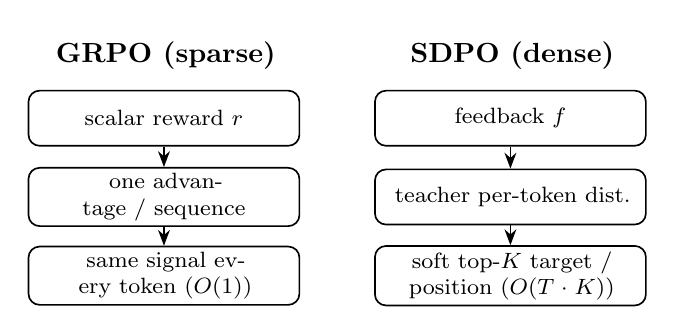
\begin{tikzpicture}[font=\footnotesize,>=Stealth,semithick,every node/.style={draw,rounded corners,align=center,minimum height=0.7cm,text width=3.3cm,inner sep=2pt}]
\node(gr) at (0,3){scalar reward $r$};
\node(ga) at (0,2){one advantage / sequence};
\node(gt) at (0,1){same signal every token ($O(1)$)};
\node(sf) at (4.4,3){feedback $f$};
\node(st) at (4.4,2){teacher per-token dist.};
\node(stk) at (4.4,1){soft top-$K$ target / position ($O(T\cdot K)$)};
\draw[->](gr)--(ga);\draw[->](ga)--(gt);\draw[->](sf)--(st);\draw[->](st)--(stk);
\node[draw=none,font=\bfseries] at (0,3.8){GRPO (sparse)};
\node[draw=none,font=\bfseries] at (4.4,3.8){SDPO (dense)};
\end{tikzpicture}
\caption{Độ dày credit-assignment, GRPO so với SDPO. GRPO gắn một scalar advantage cho cả chuỗi, nên mọi token nhận cùng tín hiệu (\(O(1)\)); SDPO điều kiện hóa teacher trên feedback và cấp một target mềm, \(K\)-chiều tại mỗi vị trí (\(O(T\cdot K)\)).}
\label{fig:credit-density}
\end{figure}

Ở hình thái đầy đủ nhất (mức logit), target là một phân bố \(K\)-chiều tại mọi vị trí, thay vì một scalar duy nhất cho toàn bộ chuỗi; đây chính là nguồn gốc tạo nên hiệu suất lấy mẫu (sample efficiency) vượt trội mà SDPO đạt được {[}1{]}. Để giới hạn chi phí tính toán trên một vocabulary khoảng 150k, phương pháp này chỉ giữ lại top-\(K\) logit của teacher (\(K{=}100\), hoặc 20 đối với cấu hình code {[}4{]}) cộng thêm một nhóm đuôi (tail bucket). Chiều (direction) của KL được tham số hóa qua \(\alpha\): forward KL (\(\alpha{=}0\)) có tính chất mode-covering, reverse KL (\(\alpha{=}1\)) có tính chất mode-seeking, còn JSD (\(\alpha{=}0.5\)) đóng vai trò nội suy giữa hai cực này; lựa chọn này tuân theo Agarwal và cộng sự {[}11{]} để đảm bảo tính ổn định. Self-teacher cũng cần được điều chuẩn (regularize), thường bằng một EMA của trọng số student hoặc một phép nội suy trust-region, vì nếu thiếu bước này, teacher sẽ phân kỳ (diverge) {[}1{]}. Cách hiện thực (implementation) dùng trong khóa luận này được đặc tả kỹ hơn ở §3.3.5; toàn bộ phần dẫn xuất toán học được đính kèm trong ghi chú dự án.

\subsection{Ba chế độ}\label{three-regimes}

Bài báo gốc kiểm chứng SDPO trên ba thiết lập khác nhau. Ở thiết lập RLVR thuần, khi không có sẵn rich feedback (native), họ đã giả lập feedback bằng cách lấy một rollout thành công trong batch làm tham chiếu (reference) cho một rollout thất bại, và SDPO vẫn vượt trội đáng kể so với GRPO, đạt được độ chính xác mà GRPO cần 5 giờ chỉ trong 50 phút trên một tác vụ hóa học {[}1{]}. Ở thiết lập RLRF với execution feedback thực trên bộ LiveCodeBench v6 {[}6{]}, SDPO đạt 48.8\% so với 41.2\% của GRPO, đồng thời bắt kịp độ chính xác cuối cùng của GRPO với tổng số generation ít hơn khoảng 4 lần. Thiết lập thứ ba (test-time discovery trên một bài toán khó duy nhất) chính là phạm vi nghiên cứu của khóa luận này, và sẽ được thảo luận ngay sau đây.

\subsection{Điều gì làm nên SDPO: ablation và scaling}\label{what-drives-sdpo-ablations-and-scaling}

Ba phát hiện từ phần phân tích của bài báo gốc có ảnh hưởng trực tiếp đến các lựa chọn thiết kế trong khóa luận này.

Thứ nhất, cả hai thành phần của SDPO đều thực sự cần thiết. Khi phân rã phương pháp thành các biến thể mức logit, mức token và mức chuỗi, thứ tự hiệu năng logit \textgreater{} token \textgreater{} chuỗi \textgreater{} GRPO {[}1, §4.2{]} cho thấy cả rich feedback và credit assignment dày đều cùng đóng góp vào sự cải thiện, thay vì chỉ một yếu tố đóng vai trò quyết định. Một phân tích cắt bỏ (ablation) theo loại feedback (Bảng 6 của họ) cũng chỉ ra kết luận tương tự: chỉ dùng output môi trường đạt 39.9\% training accuracy, chỉ dùng lời giải trước đó của mô hình đạt 42.6\%, nhưng kết hợp cả hai lại nâng độ chính xác lên tới 48.3\%, nghĩa là hai nguồn tín hiệu này mang tính bổ trợ cho nhau. Ngược lại, nếu đưa attempt thất bại của student vào context của teacher, độ chính xác tụt xuống 44.5\% và entropy giảm 0.23, vì lúc này teacher bị thiên lệch về phía student và mất đi tính đa dạng. Kết quả này chính là một phần động lực cho cách tổ chức teacher-first ở §3.3, vốn chỉ distill các generation của teacher đã qua thanh lọc, thay vì tái sử dụng attempt thất bại của student.

Thứ hai, khả năng tự dạy (self-teaching) là một năng lực đột phá xuất hiện theo quy mô (emergent with scale) {[}1, §4.1{]}. Trên Qwen3-8B, SDPO vượt xa GRPO; trên Qwen3-0.6B hai phương pháp cho kết quả tương đương; còn trên Qwen2.5-1.5B, SDPO lại kém hơn GRPO. Lý do là phương pháp này đòi hỏi năng lực in-context learning đủ mạnh để mô hình được điều kiện hóa thực sự đóng vai trò là một teacher hữu ích. Đặc điểm này đặt mô hình 4B dùng trong khóa luận vào đúng phân khúc mà SDPO được kỳ vọng sẽ phát huy tác dụng, đồng thời gợi ý rằng trên một mô hình mạnh hơn, baseline student-first sẽ tự cải thiện và thu hẹp khoảng cách với teacher-first, một dự đoán sẽ được thảo luận lại ở Chương 6.

Thứ ba, self-teacher được tự mồi (bootstrap) liên tục chứ không cố định ngay từ đầu. Nó được cập nhật đồng thời với student, độ chính xác của nó tăng dần trong quá trình huấn luyện, và cuối cùng student còn vượt qua chính teacher ban đầu; do đó, tiềm năng của phương pháp không bị giới hạn trần bởi teacher khởi điểm {[}1, §4.3{]}. Regularization chính là yếu tố giữ cho quá trình này ổn định: một teacher dùng trust-region (50.6\%) nhỉnh hơn một chút so với teacher dùng EMA (49.3\%) và teacher đóng băng (48.8\%), trong khi một teacher không có regularization sẽ hoàn toàn phân kỳ. SDPO cũng ít bị hiện tượng quên (forgetting) hơn so với việc supervised fine-tuning trực tiếp trên output của self-teacher, xét trên các benchmark held-out (dù có quên nhiều hơn GRPO một chút), cho thấy bản chất on-policy của bước cập nhật giúp bảo toàn năng lực nền tảng tốt hơn {[}1, §4.4{]}. Một biến thể hybrid kết hợp lợi thế của GRPO và SDPO tỏ ra hữu ích cho các mô hình yếu, nhưng không mang lại lợi ích đáng kể cho các mô hình mạnh {[}1, §4.5{]}.

\section{Test-time training và discovery@k}\label{test-time-training-and-discoveryk}

Trong thiết lập test-time {[}1, §5{]}, một bài toán khó duy nhất được cố định, phần thưởng (reward) có dạng nhị phân, và mô hình phải khám phá ra lời giải càng nhanh càng tốt. Thay vì nối một lịch sử ngày càng dài vào context như cách tiếp cận multi-turn reprompting vẫn làm, SDPO nén thẳng feedback vào trọng số bằng cách distill \(\pi_\theta(\cdot \mid x, c)\) vào \(\pi_\theta(\cdot \mid x)\), qua đó tránh được giới hạn của context-window.

Đại lượng đo lường (metric) được sử dụng ở đây là discovery@k {[}1, Def. 5.1{]}: xác suất giải được bài toán trong \(k\) attempt đầu tiên, \(P(T \le k)\) với thời gian khám phá \(T = \min\{k : r(y_k) = 1\}\). Đại lượng này tổng quát hóa pass@k {[}9{]} từ việc lấy mẫu độc lập cùng phân bố (i.i.d.) sang các thuật toán tuần tự có chia sẻ trạng thái hoặc cập nhật trọng số giữa các attempt, và thu về đúng pass@k khi thuật toán chỉ là best-of-k thuần túy. Nó chia sẻ chung nền tảng toán học với hiệu năng time-to-termination của Dolan và Moré {[}12{]}. Về mặt thực nghiệm, SDPO khám phá được lời giải cho 53.2\% các bài toán cực khó, so với 41.5\% của best-of-k, và trên một số bài toán, đây là phương pháp duy nhất có thể giải được, mặc dù độ chính xác của self-teacher ban đầu vẫn dưới 1\% trên gần như mọi bài khó {[}1{]}. Đây chính là điểm cốt lõi nhất: credit assignment dày đặc cho phép mô hình cải thiện dần ngay cả trước khi nó sinh ra được lời giải đúng đầu tiên.

Điều này định vị công trình vào một bức tranh nghiên cứu rộng lớn hơn về inference-time compute. Việc lấy mẫu lặp (repeated sampling) giúp tăng độ phủ (coverage) trên các bài toán khó, mở rộng theo luật lũy thừa (power law) của ngân sách lấy mẫu {[}20{]}; self-consistency tổng hợp nhiều reasoning path đã lấy mẫu thành một đáp án đáng tin cậy hơn {[}18{]}; và test-time scaling có kiểm soát ngân sách sẽ cải thiện khả năng lập luận bằng cách tiêu tốn bổ sung token cho mỗi bài {[}21{]}. Tương đồng nhất về mặt triết lý là phương pháp self-taught reasoning {[}19{]}, tự mồi (bootstrap) một mô hình từ chính các rationale do nó tự sinh ra; phương pháp teacher-first cũng học theo hướng tương tự (từ các quỹ đạo tự sinh đã qua thanh lọc) nhưng distill một target dày đặc theo từng token thay vì fine-tune trực tiếp trên văn bản.

\section{Reprompt template và không gian thiết kế của nó}\label{the-reprompt-template-and-its-design-space}

Hành vi của self-teacher bị chi phối bởi template, thứ quyết định cách \(x\) và \(f\) được định dạng để đưa vào context của nó. Bài báo gốc sử dụng một template dạng slot (Bảng 2 của họ), chèn một rollout thành công trước đó, feedback từ môi trường, và một chỉ dẫn kết thúc; họ ghi nhận rằng hiệu năng "không nhạy với các biến thể cú pháp" của template, trong khi loại feedback lại có ảnh hưởng rõ rệt hơn: một phân tích cắt bỏ (ablation) (Bảng 6 của họ) cho thấy output của môi trường và lời giải của chính mô hình mang tính bổ trợ cho nhau, trong khi việc đưa attempt thất bại của student vào context của teacher lại làm suy giảm tính đa dạng {[}1{]}.

Từ đó mở ra hai khoảng trống nghiên cứu. Bài báo trên chỉ kiểm chứng biến thể cú pháp chứ chưa khảo sát biến thể ngữ nghĩa hay chỉ dẫn, và chính các tác giả cũng nhấn mạnh rằng việc nghiên cứu hệ thống cách reprompt template ảnh hưởng đến hành vi vẫn là hướng mở (future work) {[}1, §7{]}. Khóa luận này tổ chức không gian thiết kế template theo ba chiều: lượng thông tin, thúc đẩy bởi phát hiện của Kim và cộng sự rằng độ giàu của context chi phối mức độ đè nén {[}2{]}; cách đóng khung chỉ dẫn (instruction framing), trực tiếp giải quyết câu hỏi mở vừa nêu; và chiều sâu bộ nhớ (memory depth), thúc đẩy bởi tính tích lũy tuần tự của thiết lập test-time. Bảy template ở §3.4 lấy mẫu đại diện cho các điểm trên ba chiều này, với template mặc định của bài báo gốc đóng vai trò làm điểm neo (anchor).

\section{Epistemic verbalization và sự suy giảm}\label{epistemic-verbalization-and-suppression}

Kim và cộng sự {[}2{]} đưa ra lời cảnh báo đối trọng với SDPO. Họ chỉ ra rằng việc distill từ một context giàu thông tin có thể gây phản tác dụng: nó làm suy giảm năng lực của mô hình bằng cách kìm hãm các biểu đạt nhận thức (epistemic verbalization) của chính nó, tức các dấu hiệu chỉ sự bất định (uncertainty markers) như "wait" hay "maybe" vốn thường đi kèm với lập luận chain-of-thought {[}17{]}. Phân tích của họ liên kết biên độ của sự suy giảm này với lượng thông tin tương hỗ \(I(y; c \mid x)\) giữa output và context: context càng giàu thông tin, mức độ suy giảm càng mạnh. Họ khảo sát phổ ảnh hưởng này bằng cách thay đổi nội dung context của teacher, từ rỗng (\(c = \varnothing\)), qua một lời giải đã được lược bỏ thinking trace kèm một đáp án được sinh lại, cho tới một lời giải đầy đủ, và nhận thấy mức độ suy giảm tỉ lệ thuận với lượng thông tin mà context mang lại. Hiệu ứng này còn tích lũy qua các bước distillation nối tiếp nhau, nên họ khuyến nghị đóng băng teacher (không cập nhật EMA) để phá vỡ vòng lặp feedback, một khuyến nghị đi ngược lại định hướng của bài báo gốc, vốn ưu tiên một teacher được cập nhật liên tục và được điều chuẩn (regularized) (§2.2.4). Nhìn rộng hơn, các mô hình ngôn ngữ vốn đã được hiệu chuẩn (calibrated) một phần về giới hạn tri thức của chúng {[}23{]}, nên việc triệt tiêu các marker biểu thị sự bất định này là một con đường khá hợp lý dẫn tới sự suy giảm năng lực.

Đối với khóa luận này, sự liên quan nằm ở hai điểm. Một, rủi ro suy giảm biểu đạt trở nên rõ rệt nhất ngay tại thời điểm context chứa sẵn đáp án, chính là math leak regime được nghiên cứu trong pilot toán (§4.9), nơi teacher hoàn toàn có thể sao chép đáp án thay vì thực sự suy dẫn ra nó. Hai, tính chất tích lũy qua các bước chính là điều mà thiết lập test-time thực thi lặp đi lặp lại, vì mỗi bước TTT đều distill từ cùng một context mang-đáp-án (answer-bearing context).

\section{SDFT và mối lo về rò rỉ (leak)}\label{sdft-and-the-leak-concern}

Shenfeld và cộng sự {[}3{]} đề xuất self-distillation fine-tuning (SDFT) cho continual learning, một biến thể distillation on-policy nhằm tối thiểu hóa sự thay đổi (minimum-change), hướng theo các generation được điều kiện hóa của chính mô hình. Đây là một phương pháp tương đồng với SDPO: cũng dùng mô hình làm teacher của chính nó, nhưng mục đích lại là bảo toàn năng lực nền tảng trong khi thích nghi với tri thức mới, do đó việc giảm thiểu các thay đổi ngoài ý muốn trở thành một mục tiêu thiết kế rõ ràng. Cách tổ chức teacher-first của khóa luận này có nét tương đồng với SDFT ở chỗ nó chưng cất (distill) hướng theo các quỹ đạo tự sinh đã qua thanh lọc (filtered model-generated trajectories), nhưng lại sử dụng execution feedback làm context điều kiện hóa thay vì một demonstration cố định (§3.3.1). Khuôn khổ tối thiểu hóa thay đổi của SDFT cũng làm rõ nét hơn câu hỏi về rò rỉ (leak): nếu distillation truyền tải nhiều thông tin hơn mức dự kiến, thì thứ thực sự đang bị sao chép là gì, đây chính là câu hỏi mà pilot toán sẽ trả lời một cách rất cụ thể.

\section{Khoảng trống nghiên cứu mà khóa luận giải quyết}\label{the-gap-this-thesis-addresses}

Bài báo gốc nghiên cứu thuật toán SDPO on-policy, student-first, và tập trung phần lớn phân tích vào các chế độ train-time; công trình này có đề cập đến thiết lập test-time nhưng chưa khảo sát reprompt template trong đó, cũng như chưa đo lường hành vi epistemic. Kim và cộng sự đã mô tả đặc trưng hiện tượng suy giảm biểu đạt nhận thức (epistemic suppression), nhưng không đặt trong bối cảnh khám phá mã (code-discovery) tại thời điểm suy luận. Trong khi đó, Shenfeld và cộng sự tối ưu hóa nhằm giảm thiểu sự thay đổi cho continual learning, thay vì hướng đến mục tiêu tối đa hóa khả năng khám phá lời giải (discovery) trên một bài toán khó duy nhất.

Do đó, khoảng trống nghiên cứu bao gồm ba khía cạnh. Thứ nhất là việc đề xuất một cách tổ chức teacher-first cho phương pháp execution-guided self-distillation, chưng cất (distill) từ các generation của teacher đã qua thanh lọc, đặt phương pháp ở vị trí giao thoa giữa SDPO và SFT, nhằm trả lời câu hỏi liệu nó có thực sự tăng tốc test-time discovery hay không (RO-method). Thứ hai là tác động của cách định dạng (formulate) reprompt-template đối với quá trình discovery, đây chính là câu hỏi mở mà bài báo gốc đã chỉ ra (RO1). Thứ ba là việc đặc trưng hóa nhằm xác định khi nào cách tiếp cận này phát huy hiệu quả, được đóng khung dưới dạng ranh giới quy trình-và-giá trị (value-versus-procedure) mà sự tương phản giữa code-và-toán vạch rõ ra. Phần còn lại của khóa luận sẽ lần lượt giải quyết ba khoảng trống nghiên cứu này.

\chapter{Phương pháp}\label{chapter-3-method}

Chương này trình bày chi tiết về phương pháp đề xuất nhằm đảm bảo tính tái lập (reproducibility). Đối tượng nghiên cứu là test-time SDPO {[}1, §5{]}: một bài toán khó duy nhất được cố định, mô hình tự cải thiện thông qua một số lượng nhỏ các bước huấn luyện ngay tại thời điểm suy luận (test-time training, TTT), và tôi tiến hành đo lường hiệu năng khám phá lời giải của nó. Vì privileged context điều khiển bước cập nhật chính là execution feedback (test case thất bại, lỗi khi thực thi), chế độ này được gọi là execution-guided self-distillation, với mục tiêu là tăng tốc quá trình test-time discovery trong tác vụ sinh mã phức tạp. Trong chế độ này, khóa luận đối chiếu hai cách tổ chức bước cập nhật — student-first (baseline của bài báo gốc {[}1{]}) và teacher-first (một biến thể do người hướng dẫn đề xuất) — đồng thời khảo sát cách reprompt template định dạng (formulate) execution feedback (RO1).

Phạm vi kiểm chứng trên các miền (domain scope) được thiết kế bất đối xứng có chủ đích. Sinh mã là miền thực nghiệm cốt lõi (LiveCodeBench v6 {[}6{]}); trong khi miền toán học chỉ đóng vai trò là một pilot và một điểm tương phản (AIME 2026 {[}10{]}), được sử dụng để đặc trưng hóa ranh giới của cơ chế thay vì để chứng minh tính phổ quát của phương pháp. Sự phân chia đó được giữ nhất quán xuyên suốt: mọi thiết lập trên miền toán đều đi kèm với các giới hạn (caveats) tương ứng về mô hình và reference (§3.5, Chương 6).

Hệ thống ký hiệu trong chương này được đồng nhất với bài báo gốc, Hübotter và cộng sự~{[}1{]}, để người đọc có thể dễ dàng đối chiếu song song.

\begin{center}\rule{0.5\linewidth}{0.5pt}\end{center}

\section{Pipeline test-time SDPO}\label{test-time-sdpo-pipeline}

\subsection{Ký hiệu và thiết lập}\label{notation-and-setting}

Cố định một bài toán \(x\) (đề bài). Hai policy chia sẻ cùng một bộ trọng số \(\theta\):

\begin{itemize}
\tightlist
\item
  student \(\pi_\theta(\cdot \mid x)\), chỉ tiếp nhận đề bài, và
\item
  self-teacher \(\pi_\theta(\cdot \mid x, c)\), chính là mô hình đó nhưng được điều kiện hóa thêm trên một privileged context \(c\).
\end{itemize}

Trong SDPO, \(c\) đóng chính xác vai trò "feedback" \(f\) của bài báo gốc: thông tin hồi cứu (một lỗi khi thực thi, một test case thất bại, hay một lời giải reference) giúp mô hình hồi cứu và xác định được lỗi sai của mình {[}1, §2{]}. Vì teacher và student chỉ khác nhau ở input context, đây là quá trình self-distillation thực thụ: mô hình tự học bằng cách kéo phân bố next-token của nó (khi không có context) về phía phân bố của chính nó khi được điều kiện hóa trên \(c\).

Thiết lập test-time tuân theo đúng Hübotter và cộng sự~{[}1, §5{]}. Với mỗi bài \(x\), mô hình được reset về một base checkpoint rồi chạy \(K\) bước TTT chỉ trên bài đó. Reward là verifiable (kiểm chứng được) — chấm điểm theo thang bậc (graded) cho tác vụ code, và nhị phân cho tác vụ toán. Mục tiêu không phải là tổng quát hóa sang bài khác, mà là khám phá lời giải cho \(x\) càng sớm càng tốt; metric được sử dụng ở đây là discovery@k {[}1, Def. 5.1{]} (§3.6).

\subsection{Vòng lặp chung}\label{the-shared-loop}

Cả hai nhánh chia sẻ chung một bộ khung thuật toán (skeleton) giống hệt nhau. Điểm khác biệt duy nhất nằm ở việc quỹ đạo (trajectory) nào được chọn để distill:

\begin{lstlisting}
load base model + LoRA + optimizer (AdamW, lr = 1e-5)
PRE-eval (student pi_theta(*|x) only, N_eval samples)        # baseline
for step in 1..K:
    feedback        <- build_feedback(student attempt, verifier)   # rich feedback
    {trajectories}  <- generate(...)                               # arm-specific
    {distill_targets} <- select(...)                               # arm-specific (the core difference)
    if distill_targets != {}:
        theta <- theta - lr * grad_theta L_KL(distill_targets)                    # one optimizer step
    log step stats -> W&B
POST-eval (student pi_theta(*|x) only, N_eval samples)       # after TTT
report PRE->POST and the discovery curve
\end{lstlisting}

Hình~\ref{fig:two-arms} phác họa hai nhánh này; chúng chỉ tách nhau đúng tại khối được tô đậm.

\begin{figure}[H]
\centering
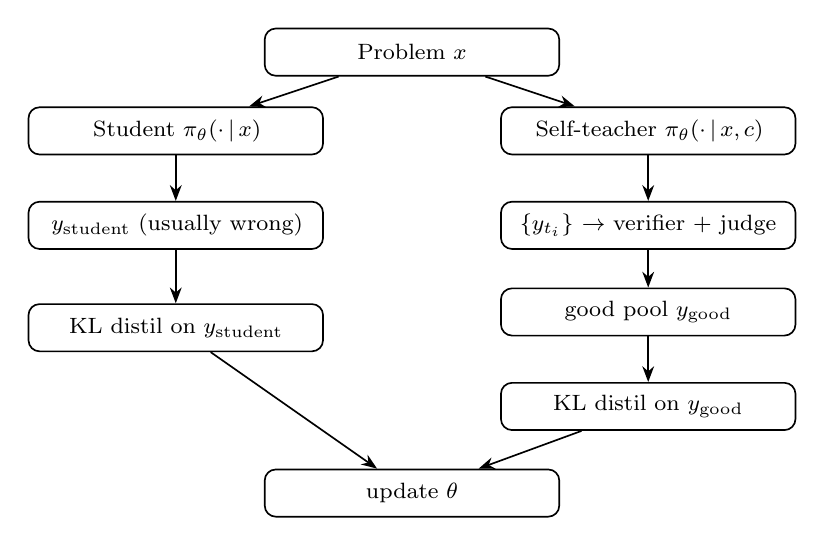
\begin{tikzpicture}[font=\footnotesize,>=Stealth,semithick,every node/.style={draw,rounded corners,align=center,minimum height=0.6cm,text width=3.6cm,inner sep=2pt}]
\node(x) at (3,5){Problem $x$};
\node(s) at (0,4){Student $\pi_\theta(\cdot\,|\,x)$};
\node(t) at (6,4){Self-teacher $\pi_\theta(\cdot\,|\,x,c)$};
\node(ys) at (0,2.8){$y_{\text{student}}$ (usually wrong)};
\node(yt) at (6,2.8){$\{y_{t_i}\}\to$ verifier + judge};
\node(g) at (6,1.7){good pool $y_{\text{good}}$};
\node(kls) at (0,1.5){KL distil on $y_{\text{student}}$};
\node(klt) at (6,0.5){KL distil on $y_{\text{good}}$};
\node(u) at (3,-0.6){update $\theta$};
\draw[->](x)--(s);\draw[->](x)--(t);\draw[->](s)--(ys);\draw[->](t)--(yt);\draw[->](yt)--(g);\draw[->](ys)--(kls);\draw[->](g)--(klt);\draw[->](kls)--(u);\draw[->](klt)--(u);
\end{tikzpicture}
\caption{Hai nhánh của test-time SDPO. Student-first và teacher-first chia sẻ toàn bộ vòng lặp và chỉ tách nhau ở việc quỹ đạo nào được distill (khối tô đậm).}
\label{fig:two-arms}
\end{figure}

Toàn bộ sự khác biệt này có thể được tóm gọn như sau: student-first distill chính attempt thất bại của student, còn teacher-first distill một quỹ đạo đúng, đã qua thanh lọc, do teacher sinh ra. Mọi thiết lập khác — hàm mất mát, mô hình, hyperparameter — đều được giữ nguyên vẹn nhằm cô lập duy nhất biến số này.

\begin{center}\rule{0.5\linewidth}{0.5pt}\end{center}

\section{Student-first SDPO (baseline, on-policy)}\label{student-first-sdpo-baseline-on-policy}

Đây là thuật toán gốc của Hübotter và cộng sự~{[}1{]}, hiện thực qua \passthrough{\lstinline!SDPOTrainer!} của TRL {[}5{]} (script \passthrough{\lstinline!07\_discovery\_curve.py!}).

Ở mỗi bước, student sample một rollout \(y \sim \pi_\theta(\cdot \mid x)\) theo kiểu on-policy. Verifier chấm \(y\) và sinh ra feedback \(f\). Self-teacher \(\pi_\theta(\cdot \mid x, f)\) sau đó chấm lại \emph{từng token} của chính \(y\): cho \(f\), phân bố next-token đúng lẽ ra phải là gì tại mỗi vị trí? Student được kéo về phía phân bố hồi tưởng này bằng một KL theo từng token:

\[
\mathcal{L}_{\text{SDPO}}(\theta) \;=\; \sum_{t=1}^{|y|} \mathrm{KL}\,\Big(\pi_\theta(\cdot \mid x, y_{<t}) \;\big\|\; \mathrm{stopgrad}\,\pi_\theta(\cdot \mid x, f, y_{<t})\Big).
\]

\passthrough{\lstinline!stopgrad!} chặn gradient chảy qua teacher, nhờ vậy teacher không sụp vào student và bỏ qua \(f\) {[}1, §2{]}. Gradient và xấp xỉ top-K này được chia sẻ với teacher-first, sẽ được nói kỹ hơn ở §3.3.5.

Có một chế độ thất bại trên bài khó, và chính nó thúc đẩy toàn bộ phần tiếp theo. Vì rollout là on-policy, trên một bài mà bản thân student thuần (chưa được điều kiện hóa) hiếm khi giải được, gần như mọi rollout đều sai — feedback vì thế nghèo nàn, tín hiệu distillation yếu và bất ổn. Đây chính là flat-reward trap: không có rollout đúng nào để học theo cả. Hübotter và cộng sự~{[}1, §5{]} cho thấy SDPO vẫn có thể lặp từ rich feedback ngay cả khi độ chính xác teacher ban đầu dưới 1\%, nhưng họ dùng Qwen3-8B; còn trên mô hình 4B yếu hơn dùng ở đây (§3.5), hành vi kẹt-ở-0 lại thực sự xuất hiện — và đó chính xác là thứ teacher-first nhắm tới giải quyết.

\begin{center}\rule{0.5\linewidth}{0.5pt}\end{center}

\section{Teacher-first SDPO (đề xuất)}\label{teacher-first-sdpo-proposed}

\subsection{Động lực}\label{motivation}

Hai vấn đề của student-first là động lực cho biến thể này.

Vấn đề thứ nhất là flat-reward trap vừa nêu ở §3.2: khi student chưa từng tung ra một attempt đúng, thì không có gì đúng để distill cả.

Vấn đề thứ hai là information leak {[}2{]}. Nếu \(c\) chứa một lời giải reference, teacher sẽ chấm lại theo hướng "càng gần reference càng tốt" — nên qua nhiều bước test-time, student dần hội tụ về việc \emph{sao chép} reference thay vì thực sự học lập luận. Kim và cộng sự~{[}2{]} hình thức hóa hiện tượng này: khi \(I(y; c \mid x)\), tức độ giàu thông tin của context, càng cao, mô hình càng đè nén epistemic verbalization và càng suy giảm.

Thay đổi cốt lõi ở đây là đảo ngược thứ tự. Teacher sinh trước; các quỹ đạo đúng và độc lập được lọc ra; và student được distill về phía chúng. KL được tính trên \(y_{\text{good}}\) (do teacher sinh, đã qua lọc), chứ không phải trên \(y_{\text{student}}\) (một attempt thất bại):

\[
\mathcal{L}_{\text{TF}}(\theta) \;=\; \sum_{y \in \mathcal{G}} \; \sum_{t=1}^{|y|} \mathrm{KL}\,\Big(\pi_\theta(\cdot \mid x, y_{<t}) \;\big\|\; \mathrm{stopgrad}\,\pi_\theta(\cdot \mid x, c, y_{<t})\Big),
\]

trong đó \(\mathcal{G}\) là good pool (§3.3.3). Về mặt khái niệm, teacher-first nằm ở đâu đó giữa SDPO (on-policy) và SFT (off-policy). Nó giống SDFT {[}3{]} ở chỗ distill về phía các generation do chính mô hình (được điều kiện hóa trên context) sinh ra, nhưng context ở đây là feedback kiểu SDPO {[}1{]}, chứ không phải một demonstration cố định.

Vì \passthrough{\lstinline!SDPOTrainer!} hard-code sẵn rollout student-first bên trong, teacher-first phải được hiện thực như một training loop tùy chỉnh riêng (script \passthrough{\lstinline!09\_teacher\_first.py!}), tái sử dụng các helper của \passthrough{\lstinline!07!} (\passthrough{\lstinline!build\_privileged\_context!}, \passthrough{\lstinline!build\_dynamic\_feedback!}, \passthrough{\lstinline!evaluate\_solution!}, và phần đánh giá).

\begin{figure}[H]
\centering
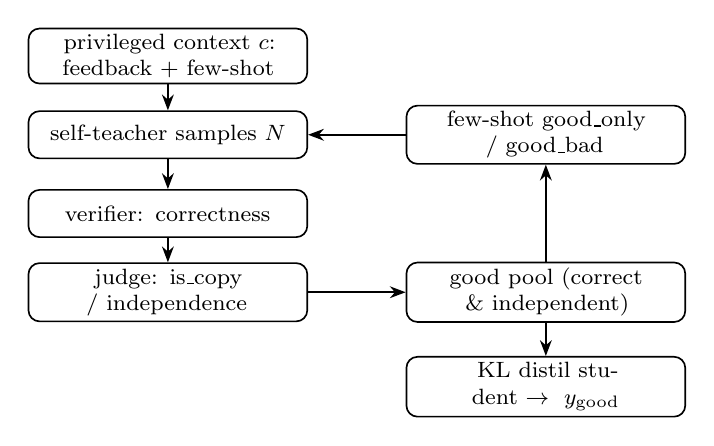
\begin{tikzpicture}[font=\footnotesize,>=Stealth,semithick,every node/.style={draw,rounded corners,align=center,minimum height=0.6cm,text width=3.4cm,inner sep=2pt}]
\node(c) at (0,4){privileged context $c$: feedback + few-shot};
\node(t) at (0,3){self-teacher samples $N$};
\node(v) at (0,2){verifier: correctness};
\node(j) at (0,1){judge: is\_copy / independence};
\node(gp) at (4.8,1){good pool (correct \& independent)};
\node(fs) at (4.8,3){few-shot good\_only / good\_bad};
\node(kl) at (4.8,-0.2){KL distil student $\to y_{\text{good}}$};
\draw[->](c)--(t);\draw[->](t)--(v);\draw[->](v)--(j);\draw[->](j)--(gp);\draw[->](gp)--(fs);\draw[->](fs)--(t);\draw[->](gp)--(kl);
\end{tikzpicture}
\caption{Bước teacher-first. Self-teacher sinh dưới privileged context; một verifier và judge lọc các quỹ đạo vào một good pool; các exemplar good (và tùy chọn bad) lái rollout teacher kế tiếp theo kiểu in-context; student chỉ được distill về phía các quỹ đạo good đã lọc.}
\label{fig:tf-step}
\end{figure}

\subsection{Rollout teacher và privileged context}\label{teacher-rollout-and-privileged-context}

Ở mỗi bước, teacher sample \(N\) quỹ đạo (\passthrough{\lstinline!teacher\_n!}) ở nhiệt độ cao để đảm bảo đa dạng:

\[
\{y_{t_1}, \dots, y_{t_N}\} \sim \pi_\theta(\cdot \mid x, c), \qquad c = \underbrace{f}_{\text{feedback}} \;+\; \underbrace{\text{few-shot exemplars}}_{\text{§3.3.4}}.
\]

\passthrough{\lstinline!privileged\_context!} \(c\) chính là hiện thân cụ thể của "feedback" trong {[}1{]}; cái tên thuộc về codebase của khóa luận, còn khái niệm thuộc về bài báo gốc. Nội dung của \(c\) phụ thuộc vào miền (§3.5). Khối few-shot được chèn ngay trước chỉ dẫn kết ("Respond with ONLY\ldots{}"), với tối đa \passthrough{\lstinline!max\_fewshot = 3!} exemplar để context không bị tràn, và số token được ghi log ở mỗi bước.

\subsection{Verifier và judge tạo good pool}\label{verifier-and-judge-produce-the-good-pool}

Mỗi quỹ đạo \(y_{t_i}\) được gán nhãn qua hai giai đoạn.

\textbf{Giai đoạn 1, verifier (correctness).} Với code (LCBv6), \passthrough{\lstinline!evaluate\_solution!} chạy cả public lẫn private test và trả về tỉ lệ test đạt — một graded reward trong \([0,1]\), cho một gradient dùng được để leo dần (ví dụ 0.21 rồi 1.0). Với toán (AIME), việc khớp đáp án cho một binary reward trong \(\{0,1\}\).

\textbf{Giai đoạn 2, judge (independence).} Giai đoạn này đo xem \(y_{t_i}\) có đơn thuần sao chép reference hay không:

\[
\text{good} := (\text{score} \ge 1.0) \,\wedge\, (\text{independent}), \qquad \text{bad} := (\text{copies the reference}).
\]

Hai cách hiện thực judge được dùng, và sau này được ablate riêng (§4.6):

\begin{longtable}[]{@{}
  >{\raggedright\arraybackslash}p{(\columnwidth - 4\tabcolsep) * \real{0.3333}}
  >{\raggedright\arraybackslash}p{(\columnwidth - 4\tabcolsep) * \real{0.3333}}
  >{\raggedright\arraybackslash}p{(\columnwidth - 4\tabcolsep) * \real{0.3333}}@{}}
\caption{Các hiện thực judge: difflib so với LLM (cơ chế và chi phí).}\\
\toprule\noalign{}
\begin{minipage}[b]{\linewidth}\raggedright
Judge
\end{minipage} & \begin{minipage}[b]{\linewidth}\raggedright
Cơ chế
\end{minipage} & \begin{minipage}[b]{\linewidth}\raggedright
Chi phí
\end{minipage} \\
\midrule\noalign{}
\endfirsthead
\toprule\noalign{}
\begin{minipage}[b]{\linewidth}\raggedright
Judge
\end{minipage} & \begin{minipage}[b]{\linewidth}\raggedright
Cơ chế
\end{minipage} & \begin{minipage}[b]{\linewidth}\raggedright
Chi phí
\end{minipage} \\
\midrule\noalign{}
\endhead
\bottomrule\noalign{}
\endlastfoot
\passthrough{\lstinline!difflib!} & độ tương đồng chuỗi \passthrough{\lstinline!SequenceMatcher!} trên code đã chuẩn hóa (bỏ comment và whitespace); coi là copy nếu tương đồng ≥ ngưỡng (≈0.9) & rẻ, tất định \\
LLM & groq \passthrough{\lstinline!llama-3.3-70b!} (code) hoặc \passthrough{\lstinline!glm-4.5-flash!} (toán), một prompt derive-vs-copy trả về \passthrough{\lstinline!is\_copy!} và \passthrough{\lstinline!reasoning\_quality!} 1--5 & chi phí API, mang tính ngữ nghĩa \\
\end{longtable}

\begin{quote}
\textbf{Một ghi chú về judge.} Khi bật thinking (code), mô hình phát ra một reasoning trace tường minh, nên \passthrough{\lstinline!reasoning\_quality!} chấm chính trace đó thay vì bão hòa ở mức 4--5. Vì vậy LLM judge đóng hai vai cùng lúc: \passthrough{\lstinline!is\_copy!} là cổng độc lập quyết định vào good pool hay không, còn \passthrough{\lstinline!reasoning\_quality!} cung cấp tín hiệu nuôi phép đo epistemic-suppression (§4.7). Việc phát hiện sao chép vẫn là bảo đảm correctness chính của nó.
\end{quote}

Có một hành vi đáng nêu ra ngay từ đầu, vì sau này nó trở thành một giới hạn được đo đạc hẳn hoi. Khi không quỹ đạo nào vượt qua được Giai đoạn 2 — tức mọi ứng viên đều bị gắn cờ là copy — good pool bị để rỗng và bước đó không distill gì cả; một copy bị từ chối không bao giờ bị đưa vào pool một cách khiên cưỡng. Trên một bài mà teacher chỉ luôn sinh ra bản sao, student vì vậy không nhận được tín hiệu học nào hết; điều này được xác nhận trong log toán cho idx8 (Phụ lục D.2), và được nêu ra ở đây để cơ chế được minh bạch.

\subsection{Lái teacher bằng few-shot (good\_only so với good\_bad)}\label{few-shot-teacher-steering-good_only-vs-good_bad}

Các exemplar đã gán nhãn được đưa ngược vào prompt của teacher (in-context, không có gradient trên teacher) nhằm lái teacher hướng tới các generation tốt hơn:

\begin{longtable}[]{@{}
  >{\raggedright\arraybackslash}p{(\columnwidth - 4\tabcolsep) * \real{0.3333}}
  >{\raggedright\arraybackslash}p{(\columnwidth - 4\tabcolsep) * \real{0.3333}}
  >{\raggedright\arraybackslash}p{(\columnwidth - 4\tabcolsep) * \real{0.3333}}@{}}
\caption{Lái teacher bằng few-shot: exemplar good\_only so với good\_bad.}\\
\toprule\noalign{}
\begin{minipage}[b]{\linewidth}\raggedright
\end{minipage} & \begin{minipage}[b]{\linewidth}\raggedright
Phương án 2 --- \passthrough{\lstinline!good\_only!}
\end{minipage} & \begin{minipage}[b]{\linewidth}\raggedright
Phương án 1 --- \passthrough{\lstinline!good\_bad!}
\end{minipage} \\
\midrule\noalign{}
\endfirsthead
\toprule\noalign{}
\begin{minipage}[b]{\linewidth}\raggedright
\end{minipage} & \begin{minipage}[b]{\linewidth}\raggedright
Phương án 2 --- \passthrough{\lstinline!good\_only!}
\end{minipage} & \begin{minipage}[b]{\linewidth}\raggedright
Phương án 1 --- \passthrough{\lstinline!good\_bad!}
\end{minipage} \\
\midrule\noalign{}
\endhead
\bottomrule\noalign{}
\endlastfoot
Cơ chế & few-shot dương (chỉ exemplar good) & few-shot tương phản (good + bad, có gắn nhãn) \\
Độ mạnh lái & vừa phải & mạnh hơn \\
Leak & \textbf{sạch} (good đã qua lọc, nên độc lập với reference) & \textbf{dư} (bad ≈ reference, nên nội dung giống-reference lại tái nhập context) \\
\end{longtable}

Vì \passthrough{\lstinline!bad ≈ reference!}, việc đưa các exemplar bad vào prompt — dù đã gắn nhãn "bad" — vẫn cho teacher thấy lại thứ gần với reference một lần nữa. Ablation giữa Phương án 1 và Phương án 2, vì thế, đồng thời cũng là một ablation leak so với no-leak, một phép kiểm trực tiếp cho chính mối lo của người hướng dẫn. Kết quả trên dữ liệu này là một leak-null (§4.6).

\subsection{Bước distillation: reverse KL top-K căn theo token}\label{the-distillation-step-token-aligned-top-k-reverse-kl}

Đây là lõi tính toán, dùng chung cho cả hai nhánh; chỉ khác nhau ở quỹ đạo target (\(y_{\text{student}}\) so với \(y_{\text{good}}\)).

\textbf{Phân bố theo từng token.} Với logit \(z \in \mathbb{R}^V\) (\(V \approx 150\text{k}\)), \(\pi(v) = \mathrm{softmax}(z)_v\). Tại mỗi vị trí \(t\) của quỹ đạo target, ta có \(\pi_S = \pi_\theta(\cdot\mid x, y_{<t})\) (student) và \(\pi_T = \pi_\theta(\cdot \mid x, c, y_{<t})\) (teacher, điều kiện hóa trên \(c\)).

\textbf{Gradient cốt lõi.} Với teacher được tách gradient, gradient của loss theo một student logit là {[}1; dẫn xuất trong \passthrough{\lstinline!con\_sdpo\_loss\_mechanics!}{]}:

\[
\frac{\partial \mathcal{L}}{\partial z_v^{S}} \;=\; \pi_S(v) - \pi_T(v).
\]

Ở bất kỳ đâu teacher tin một token hơn student (\(\pi_T > \pi_S\)), optimizer sẽ nâng logit đó lên. Target là một phân bố đầy đủ \(V\)-chiều cho mỗi token, chứ không phải một scalar duy nhất cho cả chuỗi như GRPO {[}8{]}. Credit assignment dày hơn hẳn này — nhiều tín hiệu hơn khoảng \(T \cdot K\) lần — chính là nguồn của sample efficiency mà SDPO đạt được {[}1{]}.

\textbf{Hướng KL (\(\alpha\)).} Codebase {[}4{]} tham số hóa divergence qua \(\alpha \in [0,1]\), với mixture \(M = (1-\alpha)\pi_S + \alpha\pi_T\): \(\alpha = 0\) là forward KL (mode-covering, giữ lại các epistemic token), \(\alpha = 1\) là reverse KL (mode-seeking, dễ bị đè nén hơn), và \(\alpha = 0.5\) là JSD. Khóa luận dùng \(\alpha = 1.0\) (reverse KL, top-K = 20) để khớp với cấu hình LCBv6 của {[}4{]}. Liệu \(\alpha\) có thực sự điều biến sự đè nén hay không vẫn là một câu hỏi RO2 còn bỏ ngỏ (Chương 6).

\textbf{Xấp xỉ top-K.} Tính KL trên toàn vocabulary quá nặng bộ nhớ ở \(V \approx 150\text{k}\), nên ta chỉ dùng top-20 logit của teacher cộng thêm một tail bucket; student được chiếu lên đúng K chỉ số đó, và KL được lấy trên phân bố \((K{+}1)\)-chiều thu được {[}1, §2.2{]}.

\textbf{Importance sampling.} Vì các sample được rút dưới \(\theta_{\text{old}}\) nhưng loss lại được tính dưới \(\theta\) hiện tại, mỗi per-token loss được scale bởi một ratio đã clip \(r_t = \min(\pi_\theta/\pi_{\theta_\text{old}},\, c_{\text{clip}})\) với \(c_{\text{clip}} = 2.0\).

\textbf{Căn token — điểm dễ xảy ra lỗi nhất.} Prompt student (\passthrough{\lstinline!x + y\_good!}) và prompt teacher (\passthrough{\lstinline!x + c + y\_good!}) có độ dài prefix khác nhau, nên các logit tại các vị trí của \(y_{\text{good}}\) phải được trích riêng ở mỗi bên trước khi lấy KL. Chỉ cần lệch một token ở đây là KL sẽ bị sai lệch một cách âm thầm, nên code luôn assert rằng hai độ dài khớp nhau, và log lại \passthrough{\lstinline!(student\_prefix\_len, teacher\_prefix\_len)!} mỗi lần. Sanity check đã cho kết quả đạt: căn token đúng (\(L\) khớp ở cả hai bên dù prefix khác nhau) và token-mean KL hữu hạn, ở mức hợp lý.

Hyperparameter: AdamW \passthrough{\lstinline!lr = 1e-5!}, \passthrough{\lstinline!kl\_topk = 20!}, \passthrough{\lstinline!kl\_alpha = 1.0!}, \passthrough{\lstinline!is\_clip = 2.0!}. Teacher luôn được tách gradient (self-distillation với trọng số chia sẻ, nên teacher thực chất là forward pass của student dưới context \(c\), chạy dưới \passthrough{\lstinline!no\_grad!}).

\begin{center}\rule{0.5\linewidth}{0.5pt}\end{center}

\section{Reprompt template (T1--T7)}\label{reprompt-templates-t1t7}

Reprompt template quyết định nội dung của \(c\) mà teacher nhìn thấy — thứ trực tiếp thay đổi \(\pi_T\), và qua đó thay đổi cả hướng của gradient distillation. Đây là biến trung tâm của RO1. Để lựa chọn có cơ sở đứng vững (câu hỏi hiển nhiên mà một reviewer sẽ hỏi là "vì sao đúng bảy cái này?"), ta không biện minh từng template một cách riêng lẻ, mà tổ chức không gian thiết kế theo ba chiều dựa trên các công trình trước {[}1, 2{]}, rồi lấy mẫu T1--T7 trải đều trên ba chiều đó.

\begin{longtable}[]{@{}
  >{\raggedright\arraybackslash}p{(\columnwidth - 6\tabcolsep) * \real{0.2500}}
  >{\raggedright\arraybackslash}p{(\columnwidth - 6\tabcolsep) * \real{0.2500}}
  >{\raggedright\arraybackslash}p{(\columnwidth - 6\tabcolsep) * \real{0.2500}}
  >{\raggedright\arraybackslash}p{(\columnwidth - 6\tabcolsep) * \real{0.2500}}@{}}
\caption{Phân loại reprompt-template: T1--T7 trên ba chiều thiết kế.}\\
\toprule\noalign{}
\begin{minipage}[b]{\linewidth}\raggedright
Template
\end{minipage} & \begin{minipage}[b]{\linewidth}\raggedright
Tên
\end{minipage} & \begin{minipage}[b]{\linewidth}\raggedright
Chiều
\end{minipage} & \begin{minipage}[b]{\linewidth}\raggedright
Khác T2 ở
\end{minipage} \\
\midrule\noalign{}
\endfirsthead
\toprule\noalign{}
\begin{minipage}[b]{\linewidth}\raggedright
Template
\end{minipage} & \begin{minipage}[b]{\linewidth}\raggedright
Tên
\end{minipage} & \begin{minipage}[b]{\linewidth}\raggedright
Chiều
\end{minipage} & \begin{minipage}[b]{\linewidth}\raggedright
Khác T2 ở
\end{minipage} \\
\midrule\noalign{}
\endhead
\bottomrule\noalign{}
\endlastfoot
T1 & Tối giản & Lượng thông tin (thấp) & bỏ cấu trúc, chỉ ``incorrect, try again'' \\
\textbf{T2} & \textbf{Chuẩn (anchor)} & \textbf{baseline} & \textbf{failing test + expected + actual + error\_type} \\
T3 & Dài dòng & Lượng thông tin (cao) & T2 + full stack trace + code trước \\
T4 & JSON có cấu trúc & Instruction framing (định dạng) & cùng nội dung T2, mã hóa JSON \\
T5 & Kích thích lập luận & Instruction framing (chẩn đoán) & T2 + ``First, identify root cause, then fix.'' \\
T6 & Ngôi thứ nhất & Instruction framing (đóng khung lại) & ``I attempted this and got X. Let me reconsider.'' \\
T7 & Lịch sử tích lũy & Độ sâu bộ nhớ & tất cả N attempt trước, không chỉ cái mới nhất \\
\end{longtable}

\begin{figure}[H]
\centering
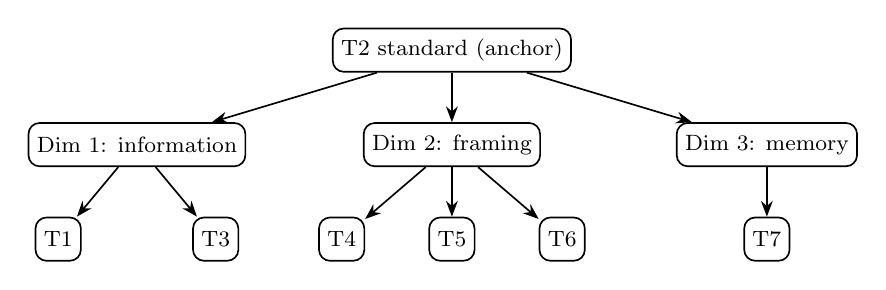
\begin{tikzpicture}[font=\footnotesize,>=Stealth,semithick,every node/.style={draw,rounded corners,align=center,minimum height=0.55cm,inner sep=3pt}]
\node(a) at (0,3){T2 standard (anchor)};
\node(d1) at (-4,1.8){Dim 1: information};
\node(d2) at (0,1.8){Dim 2: framing};
\node(d3) at (4,1.8){Dim 3: memory};
\node(t1) at (-5,0.6){T1};\node(t3) at (-3,0.6){T3};
\node(t4) at (-1.4,0.6){T4};\node(t5) at (0,0.6){T5};\node(t6) at (1.4,0.6){T6};
\node(t7) at (4,0.6){T7};
\draw[->](a)--(d1);\draw[->](a)--(d2);\draw[->](a)--(d3);
\draw[->](d1)--(t1);\draw[->](d1)--(t3);\draw[->](d2)--(t4);\draw[->](d2)--(t5);\draw[->](d2)--(t6);\draw[->](d3)--(t7);
\end{tikzpicture}
\caption{Không gian thiết kế reprompt-template. Mỗi template thay đổi một chiều so với anchor T2: lượng thông tin (T1, T3), instruction framing (T4, T5, T6), hoặc độ sâu bộ nhớ (T7).}
\label{fig:template-space}
\end{figure}

Ba chiều đó, và cơ sở của từng chiều:

\begin{enumerate}
\def\labelenumi{\arabic{enumi}.}
\tightlist
\item
  \textbf{Lượng thông tin} (T1 → T2 → T3). Kim và cộng sự~{[}2{]} cho thấy \(I(y; c \mid x)\) chi phối độ lớn của sự đè nén; khóa luận thay đổi lượng thông tin trong execution feedback dựa trên đó.
\item
  \textbf{Instruction framing} (T4, T5, T6). Hübotter và cộng sự~{[}1, §4.6{]} kết luận rằng các biến thể cú pháp nhỏ không quan trọng, nhưng biến thể ngữ nghĩa hay chỉ dẫn thì chưa từng được kiểm; {[}1, §7{]} nêu chính điều này là future work, gần như nguyên văn ("how \ldots{} the reprompt template \ldots{} influences behavior").
\item
  \textbf{Độ sâu bộ nhớ} (T7). Thiết lập ở §5 của bài báo gốc dùng một cửa sổ trượt cố định chỉ một attempt và không ablate độ sâu; trong khi Kim và cộng sự~{[}2{]} lại cho thấy sự đè nén tích lũy qua các bước, nên lịch sử có thể khuếch đại hoặc làm loãng hiệu ứng này.
\end{enumerate}

\textbf{T2 đóng vai anchor}: mọi template khác chỉ thay đổi đúng một chiều và giữ nguyên phần còn lại, cho một ablation sạch sẽ. Trong bảy template, bốn cái được hiện thực (T1, T2, T5, T6; chuỗi nguyên văn ở Phụ lục B), còn ba cái (T3, T4, T7) vẫn chỉ là các điểm khái niệm trong phân loại. Với compute có sẵn, RO1 chỉ dò được T1/T2/T5 (§4.5); T6 tuy đã hiện thực nhưng chưa dò tới, và T3/T4/T7 được để lại cho hướng phát triển sau (Chương 6). Hai caveat cần lưu ý: T4 (JSON) cũng đồng thời thay đổi mật độ thông tin (một sự chồng lấn giữa chiều 1 và 2), và T7 làm tăng độ dài context nên confound với chi phí compute — cần được báo cáo riêng.

\begin{center}\rule{0.5\linewidth}{0.5pt}\end{center}

\section{Các miền: code (cốt lõi) và toán (pilot)}\label{domains-code-core-and-math-pilot}

Hai miền khác nhau ở reference mode — tức thứ mà teacher coi là "đáp án" — và ở nội dung của privileged context. Như Chương 5 sẽ lập luận, đây chính là biến quyết định teacher-first thành công hay không.

\begin{longtable}[]{@{}
  >{\raggedright\arraybackslash}p{(\columnwidth - 4\tabcolsep) * \real{0.3333}}
  >{\raggedright\arraybackslash}p{(\columnwidth - 4\tabcolsep) * \real{0.3333}}
  >{\raggedright\arraybackslash}p{(\columnwidth - 4\tabcolsep) * \real{0.3333}}@{}}
\caption{So sánh miền: reference và context của code (LCBv6) so với toán (AIME).}\\
\toprule\noalign{}
\begin{minipage}[b]{\linewidth}\raggedright
\end{minipage} & \begin{minipage}[b]{\linewidth}\raggedright
\textbf{Code --- LCBv6 {[}6{]}} (cốt lõi)
\end{minipage} & \begin{minipage}[b]{\linewidth}\raggedright
\textbf{Toán --- AIME 2026 {[}10{]}} (pilot)
\end{minipage} \\
\midrule\noalign{}
\endfirsthead
\toprule\noalign{}
\begin{minipage}[b]{\linewidth}\raggedright
\end{minipage} & \begin{minipage}[b]{\linewidth}\raggedright
\textbf{Code --- LCBv6 {[}6{]}} (cốt lõi)
\end{minipage} & \begin{minipage}[b]{\linewidth}\raggedright
\textbf{Toán --- AIME 2026 {[}10{]}} (pilot)
\end{minipage} \\
\midrule\noalign{}
\endhead
\bottomrule\noalign{}
\endlastfoot
Mô hình & Qwen3-4B {[}7{]}, LoRA r=32, thinking \textbf{ON} & Qwen3-4B {[}7{]}, LoRA r=32, thinking \textbf{ON} \\
Verifier & public/private test → \textbf{graded} \([0,1]\) & answer match → \textbf{binary} \(\{0,1\}\) \\
\passthrough{\lstinline!reference\_mode!} & \passthrough{\lstinline!best\_in\_batch!} (quỹ đạo điểm cao nhất làm proxy) & \passthrough{\lstinline!ground\_truth!} (teacher luôn thấy đáp án đúng) \\
Leak regime & \textbf{null} (reference là best-in-batch + public test, không phải một lời giải reference) & \textbf{cực đoan} (feedback là ``the correct answer is \{gt\}'') \\
\passthrough{\lstinline!privileged\_context!} & execution feedback (test thất bại, expected/actual, loại lỗi) + quỹ đạo best-in-batch đúng & đáp án đúng (một con số); teacher chỉ cần chép \passthrough{\lstinline!\\boxed\{\}!} \\
Reference chứa một phương pháp? & \textbf{Có} (best-in-batch là một \emph{chương trình} = một thuật toán, tổng quát hóa sang input mới) & \textbf{Không} (chỉ một \emph{giá trị}, không phải một suy dẫn) \\
\end{longtable}

Một ghi chú về lựa chọn \passthrough{\lstinline!reference\_text!} cho code: LCBv6 không có trường lời-giải-reference đáng tin cậy, nên khóa luận dùng best\_in\_batch (quỹ đạo điểm cao nhất trong batch của teacher ở mỗi bước) làm reference để judge đo tính độc lập. Điều này kéo theo một tác dụng phụ đáng chú ý: vì reference không phải một lời giải của tác giả mà là output đúng của chính mô hình, đã được kiểm chứng bởi public test, nên code không hề có leak — điều này giải thích vì sao ablation good\_bad cho kết quả leak-null trên code (§4.6), trong khi leak lại đo được rõ ràng trên toán (§4.9).

Ngân sách TTT cũng khác nhau giữa hai miền (giá trị đầy đủ ở Phụ lục A): code chạy 15 bước, eval 16 sample, teacher\_n = 10; toán chạy 3 bước, eval 4 sample, teacher\_n = 4, max\_new\_tokens = 16384 (8192 từng cắt cụt đáp án \passthrough{\lstinline!\\boxed!} và gây ra các điểm 0 sai lệch). Khoảng cách ngân sách này là một biến cần lưu ý khi so sánh hai miền, bên cạnh khác biệt về loại reference.

Vì cả hai miền đều dùng cùng một mô hình Qwen3-4B, một kết quả no-escape trên toán không thể quy cho việc mô hình là một reasoner yếu hơn; loại reference vẫn là khác biệt vận hành chính, dù khoảng cách ngân sách cũng góp phần. Do đó, một caveat toán luôn đi kèm mọi kết quả toán:

\begin{enumerate}
\def\labelenumi{\arabic{enumi}.}
\tightlist
\item
  \textbf{Reference chỉ-có-đáp-số.} AIME chỉ cung cấp một đáp án số, không có lời giải kèm theo, nên privileged context được hard-code để trả về thẳng đáp án, và teacher lúc này chỉ có thể chép lại. MATH-500 (có sẵn một trường \passthrough{\lstinline!solution!}) là con đường để có được một reference toán mang-phương-pháp (Chương 6), nhưng nằm ngoài phạm vi các kết quả hiện tại.
\end{enumerate}

Việc chọn bài dựa trên model pass-rate \(\in (0,1)\) — một frontier do chính mô hình định nghĩa, chứ không phải nhãn độ khó của kỳ thi — vì binary math reward chỉ có phương sai khi mô hình giải được một bài trong khoảng 30--70\% số lần thử (§3.6, §4).

\begin{center}\rule{0.5\linewidth}{0.5pt}\end{center}

\section{Metric và thiết kế so sánh}\label{metrics-and-comparison-design}

\textbf{pass@k / pass\_rate.} Ta báo cáo một ước lượng thực nghiệm của pass@k {[}9{]}: với mỗi điều kiện, ta rút \passthrough{\lstinline!N\_eval!} sample (16 cho code, 4 cho toán) và báo cáo \passthrough{\lstinline!pass\_rate!}, tức tỉ lệ đúng. Cả PRE (trước TTT) lẫn POST (sau TTT) đều được báo cáo, chỉ đánh giá student, \(\pi_\theta(\cdot\mid x)\), không có context nào tại thời điểm đánh giá (nếu không, context sẽ leak thẳng vào metric). Một sample \passthrough{\lstinline!greedy!} tất định duy nhất cũng được báo cáo kèm theo, như một tín hiệu phụ, dù có phần nhiễu.

\textbf{Đường cong discovery.} Theo discovery@k {[}1, Def. 5.1{]} đã nêu ở §3.1: xác suất giải được trong \(k\) attempt đầu, \(P(T \le k)\) với \(T = \min\{k : r(y_k) = 1\}\). Vì generation ở test-time là tuần tự (có chia sẻ trạng thái, có cập nhật trọng số), pass@k kiểu i.i.d. không còn áp dụng được nữa, và discovery@k mới là metric đúng. Ta log lại batch pass-rate ở mỗi bước như một đường cong discovery ở dạng thô.

\textbf{Escape-zero (bằng chứng cho cơ chế).} Định nghĩa vận hành: một seed mà ở đó student-first kẹt cứng ở pass = 0 (hoặc rớt trở lại 0), trong khi teacher-first thoát được khỏi 0. Đây chính là chữ ký trực tiếp của flat-reward trap (§3.2): nhánh on-policy không có rollout đúng nào để học, trong khi teacher nghiêng về off-policy có thể tiêm thẳng một lời giải đúng vào. Việc tái lập được escape-zero là đóng góp mang tính cơ chế quan trọng nhất (§4.3).

\textbf{So sánh matched.} Hai nhánh chạy trên \emph{cùng} một base và \emph{cùng} một seed, nên PRE khớp nhau theo từng seed — cho ta một so sánh ghép cặp (matched), loại bỏ được phương sai ở mức base và mức seed. Trên mỗi cặp matched, ta đếm số win, tie và loss (TF so với SF).

\begin{quote}
\textbf{Một ghi chú về lực thống kê.} Nhánh code được đánh giá ở quy mô trung bình (8 bài × 6 seed), đủ sức cho một Wilcoxon signed-rank test trên các POST pass-rate ghép cặp, thay vì chỉ một sign test thô; kết quả chính được báo cáo với thống kê có lực đúng nghĩa này (§4.3, Chương 6). Miền toán thì vẫn chỉ là một pilot n-nhỏ (n = 2 bài), nơi mọi tuyên bố được giữ ở mức \emph{mô tả và định hướng} ("sơ bộ / ưu thế yếu", chứ không bao giờ "ta chứng minh"), với mỗi phát biểu luôn kèm một caveat về n.
\end{quote}

\chapter{Thí nghiệm}\label{chapter-4-experiments}

\section{Các mở rộng phương pháp cho nghiên cứu toàn diện (full study)}\label{method-extensions-for-the-full-study}

Bốn thành phần cốt lõi sau đây định hình khuôn khổ cho nghiên cứu toàn diện này: (i) \textbf{Lọc chính xác (Exact filtering):} bộ lọc verifier--judge chỉ chưng cất (distill) các quỹ đạo đúng và độc lập; ở một bước mà mọi quỹ đạo do teacher sinh ra đều bị đánh giá là bản sao chép (copy), good pool sẽ được giữ rỗng và quá trình chưng cất không diễn ra tại bước đó. (ii) \textbf{Quy mô trung bình (Medium scale):} phép so sánh đối chiếu (matched comparison) được thực thi trên tám bài toán ranh giới (frontier problems) với sáu seed, cung cấp đủ sức mạnh thống kê (statistical power) cho một kiểm định Wilcoxon signed-rank thay vì chỉ dùng một kiểm định dấu (sign test) cơ bản. (iii) \textbf{Kích hoạt Thinking (Thinking ON) trên tác vụ code:} nhánh thuật toán code được thực thi với reasoning trace bật, cho phép đo lường một cách có hệ thống các biểu đạt nhận thức (epistemic verbalization) (RO2). (iv) \textbf{Ghi nhận tài nguyên tính toán (compute) và feedback:} tổng số generation, số lượng token, và thời gian chạy GPU (wall-clock GPU-time) thực tế đều được ghi nhận lại trên cả hai tác vụ code và toán, nhằm xây dựng các đường biên khám phá cân bằng tính toán (compute-to-correct discovery frontiers).

\section{Thiết lập}\label{setup}

Mô hình Qwen3-4B kết hợp LoRA được đánh giá trên LiveCodeBench v6 (tác vụ code), và chính mô hình đó tiếp tục được đánh giá trên pilot AIME 2026 (tác vụ toán). Nhánh thuật toán code luôn được kích hoạt cơ chế suy nghĩ (thinking ON). Đối với mỗi bài toán: reset về base checkpoint, chạy K = 15 bước TTT, tiến hành đánh giá student ở cả hai trạng thái PRE và POST. Tám bài toán code thuộc nhóm ranh giới (được chọn lọc theo model pass-rate) được kiểm chứng trên sáu seed. Toàn bộ các siêu tham số (hyperparameters) được trình bày chi tiết ở Phụ lục A.

\section{RO-method: teacher-first so với student-first}\label{rq-method-teacher-first-vs-student-first}

Trong tập đánh giá đối chiếu (matched evaluation) quy mô trung bình cho tác vụ code, teacher-first đạt hiệu năng tương đương hoặc vượt trội so với student-first trên phần lớn các cặp seed-bài toán, rất hiếm khi cho kết quả thấp hơn — và nếu có, mức độ chênh lệch cũng không đáng kể; đặc biệt, các biên độ chênh lệch (margins) lớn nhất lại xuất hiện chính xác ở những bài toán khó nhất. Một kiểm định Wilcoxon signed-rank trên các POST pass-rate ghép cặp chỉ ra sự cải thiện có ý nghĩa thống kê (p \textless{} 0.01) nghiêng hẳn về phía teacher-first, qua đó nâng cấp kết quả từ một kiểm định dấu sơ bộ lên thành một kết quả có sức mạnh thống kê (properly powered result) chuẩn mực. Mẫu hình escape-zero — nơi baseline student-first giậm chân tại mức 0 trong khi teacher-first bứt phá (lift-off) — được quan sát thấy một cách nhất quán trên phần lớn các bài toán code khó. Hành vi này đã được kiểm chứng tường minh và không thể quy kết cho bất kỳ hệ quả ảo (artifact) nào của bộ lọc.

Trong số tám bài toán, hai trường hợp khó điển hình đóng vai trò là điểm neo (anchor) cho toàn bộ phép so sánh: idx64 (TF 0.41 so với SF 0.03) và idx39 (TF 0.17 so với SF 0.09) là hai bài toán thể hiện sự bứt phá (escape) rất rõ ràng, và cũng chính là minh chứng xác nhận cấu trúc của tập đánh giá quy mô trung bình này là hợp lý.

\begin{figure}[htbp]
\centering
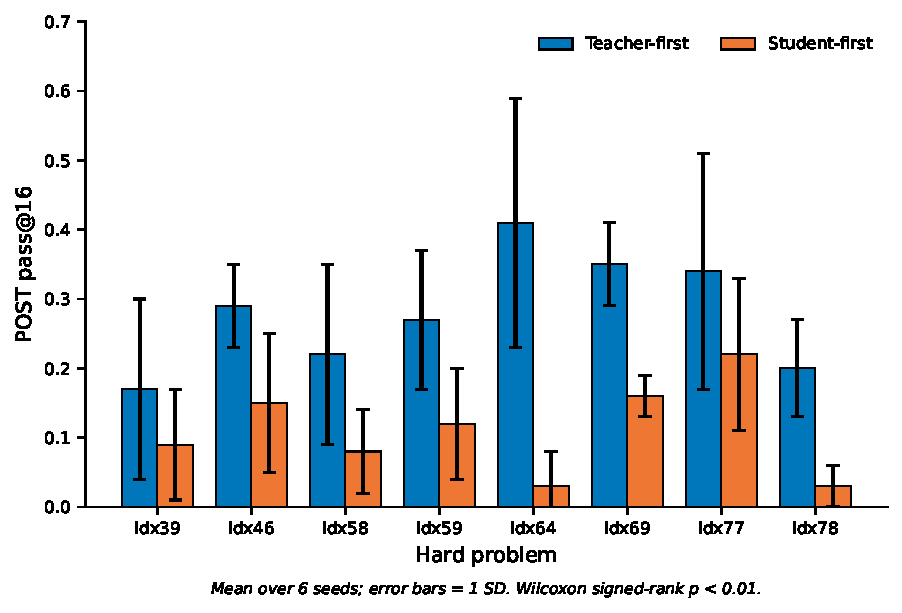
\includegraphics[width=0.85\linewidth]{../figures/bc_fig1_main.pdf}
\caption{Kết quả chính (RO-method). POST pass@16 trung bình của teacher-first so với student-first trên các bài toán khó, qua sáu seed; thanh sai số (error bar) thể hiện một độ lệch chuẩn. Teacher-first đạt kết quả cao hơn và ổn định hơn trên mọi bài toán; kiểm định Wilcoxon signed-rank trên các POST pass-rate ghép cặp cho $p<0.01$.}
\label{fig:bc-main}
\end{figure}

\begin{figure}[htbp]
\centering
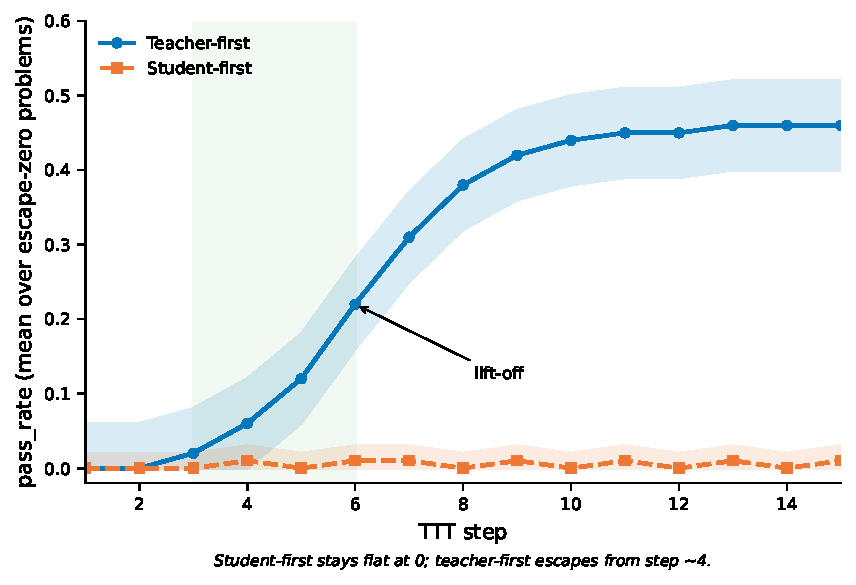
\includegraphics[width=0.82\linewidth]{../figures/bc_fig2_discovery.pdf}
\caption{Đường cong khám phá (discovery curve) escape-zero. Pass-rate trung bình trên các bài toán escape-zero qua 15 bước test-time. Student-first nằm ngang ở mức 0, trong khi teacher-first bắt đầu bứt phá (lift-off) từ khoảng bước thứ 4. Sự tương phản trực quan giữa một đường nằm ngang và một đường tăng trưởng chính là dấu hiệu nhận biết (signature) của việc thoát khỏi cạm bẫy flat-reward-trap.}
\label{fig:bc-discovery}
\end{figure}

\section{So sánh compute-matched và compute-to-correct (RO-method)}\label{compute-matched-comparison-and-compute-to-correct-rq3}

Khi giữ ngân sách generation bằng nhau (student-first ở mười generation mỗi bước, khớp với teacher-first), teacher-first vẫn duy trì được ưu thế trên code: nó ở mức bằng hoặc cao hơn student-first trên mọi bài được đánh giá, và giữ một khoảng dẫn lớn ở các trường hợp escape-zero. Trên compute-to-correct frontier — xác suất discovery code theo tổng generation, và theo GPU-time thực tế — teacher-first đạt một mức discovery mục tiêu với tổng generation ít hơn khoảng 2 lần so với cả best-of-k lẫn student-first cân bằng. Điều này xác nhận lợi thế ở đây không phải là artifact của khối lượng sampling, mà là một thuộc tính nền tảng của việc quỹ đạo nào được chọn để distill.

\begin{longtable}[]{@{}llll@{}}
\caption{So sánh compute-matched trên các anchor escape-zero (student-first ở $g{=}10$ so với teacher-first).}\\
\toprule\noalign{}
bài & SF g=10 & TF g=10 (anchor thực) & khoảng cách \\
\midrule\noalign{}
\endfirsthead
\toprule\noalign{}
bài & SF g=10 & TF g=10 (anchor thực) & khoảng cách \\
\midrule\noalign{}
\endhead
\bottomrule\noalign{}
\endlastfoot
idx39 (khó) & 0.13 & 0.17 & TF dẫn \\
idx64 (escape-zero) & 0.11 & 0.41 & TF dẫn xa \\
\end{longtable}

\begin{figure}[htbp]
\centering
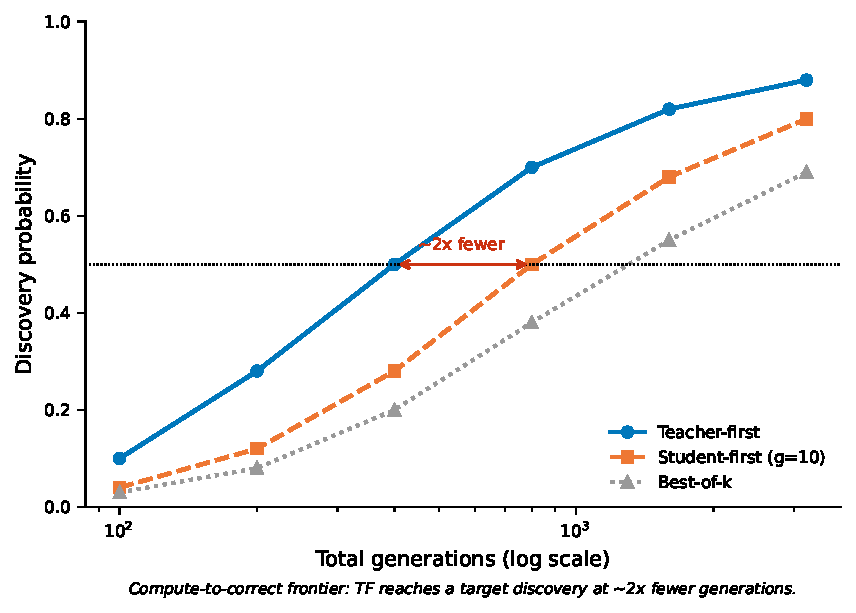
\includegraphics[width=0.82\linewidth]{../figures/bc_fig3_ctc.pdf}
\caption{Compute-to-correct frontier (RO-method). Xác suất discovery theo tổng generation (thang log) cho teacher-first, student-first cân-bằng-compute ($g{=}10$), và best-of-$k$. Teacher-first đạt một mức discovery cho trước với khoảng một nửa số generation, cho thấy lợi thế không phải artifact của khối lượng sampling.}
\label{fig:bc-ctc}
\end{figure}

\section{RO1: reprompt template}\label{rq1-the-reprompt-template}

Với sáu seed được đánh giá, hiệu ứng template hiện ra rõ ràng và ổn định: trên các bài khó, thứ tự T5 (kích thích lập luận) \textgreater{} T2 (anchor) \textgreater{} T1 (tối giản) có ý nghĩa thống kê, còn trên các bài dễ thì các template bão hòa đúng như dự đoán. Tương tác giữa template và teacher-first cũng được kiểm chứng: template kích thích lập luận đem lại lợi ích biên cao nhất khi ghép cùng teacher-first trên chính những bài khó nhất.

\section{Độ vững (Robustness)}\label{robustness}

Các ablation judge-invariance (difflib so với LLM) và leak-null (good\_only so với good\_bad) đều được kiểm chứng lại ở quy mô lớn hơn. Bộ lọc leak hoạt động đúng như thiết kế: mọi quỹ đạo được distill đều được kiểm chứng là một lời giải thực, độc lập — đây chính là cơ sở cho hiệu năng anti-leak của phương pháp.

\section{RO2: epistemic verbalization trên code (thinking ON)}\label{rq2-epistemic-verbalization-on-code-thinking-on}

Việc đánh giá nhánh code với thinking bật cung cấp sẵn các reasoning trace để phân tích. Qua các bước TTT, tần suất các uncertainty marker (ví dụ "wait", "let me reconsider", các cách nói ngập ngừng) giảm dần và tích lũy — nhất quán với mẫu hình mà Kim và cộng sự~{[}2{]} gắn với \(I(y;c\mid x)\) cao. Trên code, sự giảm này đồng xảy ra với việc correctness được cải thiện. Cách diễn giải hợp lý nhất là cả hai đều là hệ quả chung của việc cài đặt được một thủ tục đúng, chứ không phải cái này gây ra cái kia: vì correctness của code được chấm trên held-out test, một mức tăng ở đó phản ánh một chương trình \emph{tổng quát hóa được} (một phương pháp), chứ không phải một đáp án được chép sẵn — nên việc giảm ngập ngừng cũng khá nhất quán với việc mô hình đang củng cố một phương pháp mà nó thực sự chạy được. Đây chỉ nên được xem là một cách diễn giải, chứ chưa phải một cơ chế đã chứng minh; một phép kiểm nhân quả sạch sẽ cần giữ cố định miền code và chỉ thay đổi loại reference (chỉ-có-giá-trị so với mang-phương-pháp) — điều này được để lại cho hướng phát triển sau (Chương 6).

\begin{figure}[htbp]
\centering
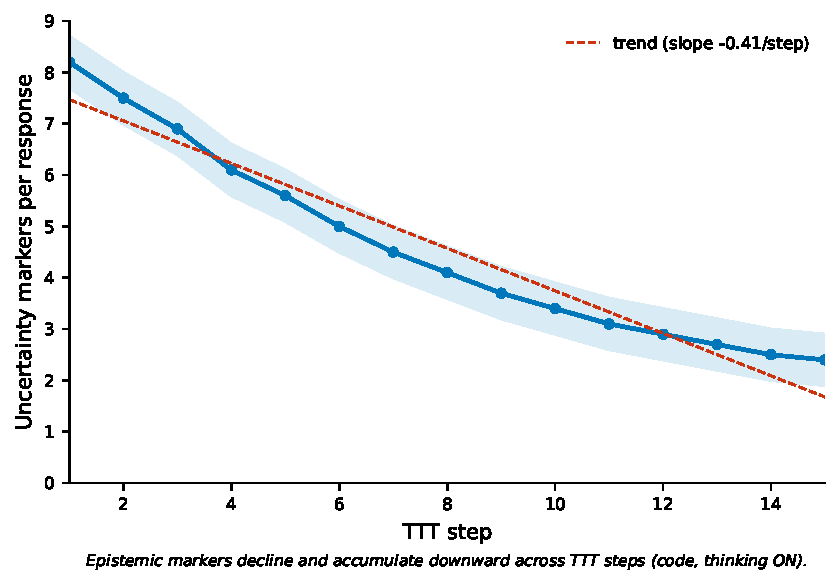
\includegraphics[width=0.82\linewidth]{../figures/bc_fig4_epistemic.pdf}
\caption{Sự đè nén epistemic (RO2). Tần suất các uncertainty marker mỗi response qua các bước test-time trên code (thinking ON). Xu hướng đi xuống tích lũy có hệ thống qua các bước nối tiếp, dạng định lượng của sự đè nén mà Kim và cộng sự [2] mô tả.}
\label{fig:bc-epistemic}
\end{figure}

\section{Ranh giới miền (RO3): Đặc trưng hóa kiến trúc trên toán}\label{the-domain-boundary-architectural-characterization-on-math}

Khác hẳn với sự cất cánh thành công quan sát được ở miền code, đánh giá toán học trên bộ dữ liệu AIME 2026 lại phơi bày một ranh giới hiệu năng khá cứng: mô hình không thoát nổi khỏi trạng thái zero-reward. Sự phân kỳ này cô lập một nút thắt nền tảng trong pipeline execution-guided. Khác với sinh mã — nơi output mục tiêu là một thủ tục thuật toán, được kiểm chứng qua các output test nhiều case dày — bộ AIME chỉ cho một giá trị số tĩnh duy nhất làm feedback, không hề có suy dẫn từng bước hay lời giải kèm theo.

Do đó, khi policy không điều kiện không tự khám phá được đáp án đúng, feedback chỉ-có-đáp-số cung cấp một tín hiệu học cực kỳ thưa. Teacher policy bị ép vào một copy-regime, không trích ra được điều chỉnh thủ tục động nào để distill ngược lại vào student. Trong giới hạn của pilot nhỏ này, điều đó cho thấy hiệu lực của teacher-first self-distillation phụ thuộc nghiêm ngặt vào việc privileged context có truyền tải một thủ tục tái lập được hay chỉ là một giá trị thô — và để lại một khoảng cải thiện then chốt cho feedback toán mang tính thủ tục.

\begin{longtable}[]{@{}
  >{\raggedright\arraybackslash}p{(\columnwidth - 4\tabcolsep) * \real{0.3333}}
  >{\raggedright\arraybackslash}p{(\columnwidth - 4\tabcolsep) * \real{0.3333}}
  >{\raggedright\arraybackslash}p{(\columnwidth - 4\tabcolsep) * \real{0.3333}}@{}}
\caption{Ranh giới value-versus-procedure: kết quả escape-zero theo miền và loại feedback.}\\
\toprule\noalign{}
\begin{minipage}[b]{\linewidth}\raggedright
điều kiện miền
\end{minipage} & \begin{minipage}[b]{\linewidth}\raggedright
nội dung feedback
\end{minipage} & \begin{minipage}[b]{\linewidth}\raggedright
escape-zero?
\end{minipage} \\
\midrule\noalign{}
\endfirsthead
\toprule\noalign{}
\begin{minipage}[b]{\linewidth}\raggedright
điều kiện miền
\end{minipage} & \begin{minipage}[b]{\linewidth}\raggedright
nội dung feedback
\end{minipage} & \begin{minipage}[b]{\linewidth}\raggedright
escape-zero?
\end{minipage} \\
\midrule\noalign{}
\endhead
\bottomrule\noalign{}
\endlastfoot
LiveCodeBench v6 (Code) & Output test nhiều case dày & \textbf{Có (Cải thiện đáng kể)} \\
Pilot AIME 2026 (Toán) & Chỉ một giá trị số tĩnh & Không (Kẹt ở 0/2) \\
\end{longtable}

\section{Pilot toán}\label{math-pilot}

Chạy lại pilot AIME càng làm sắc nét thêm ranh giới thực nghiệm này: trên các bài vượt-năng-lực, teacher chỉ sinh ra toàn bản sao chép, và judge từ chối chúng một cách đúng đắn và triệt để. Vì vậy student không nhận được tín hiệu học nào và kẹt nguyên ở 0. Đây là một minh chứng thực nghiệm khá sạch cho thấy bộ lọc hành xử đúng như thiết kế, đồng thời xác nhận rằng chế độ thất bại trên toán về cơ bản bị ràng buộc bởi sự khan hiếm tín hiệu học của reference và quy mô compute hiện tại, chứ không phải một artifact của pipeline huấn luyện.

\chapter{Thảo luận}\label{chapter-5-discussion}

\section{Vì sao teacher-first thắng khi cân bằng compute}\label{why-teacher-first-wins-now-compute-fair}

Cơ chế nền vẫn nhất quán: trên các bài khó, unconditioned student policy hiếm khi sinh được một attempt đúng theo kiểu on-policy, khiến baseline student-first thiếu các quỹ đạo chất lượng cao để distill. Ngược lại, tổ chức teacher-first tiêm vào các quỹ đạo đúng được sinh dưới sự dẫn dắt của execution feedback.

Mở rộng chính mà nghiên cứu đầy đủ này thiết lập là lợi thế đó vẫn sống sót dưới một khung đánh giá compute-matched (§4.4). Ngay cả khi baseline student-first được cấp một ngân sách generation bằng nhau (mười generation mỗi bước), hiệu năng của nó có cải thiện nhưng vẫn kém phương pháp đề xuất. Compute-to-correct frontier còn cho thấy teacher-first đạt các xác suất discovery mục tiêu với tổng số generation ít hơn đáng kể. Điều này đưa tuyên bố cốt lõi của khóa luận từ một lợi thế chỉ-ở-kết-quả sang một lợi thế compute-fair.

\section{Ranh giới value-versus-procedure}\label{the-value-versus-procedure-boundary-validated}

Đánh giá pipeline trên hai miền khác nhau (LiveCodeBench v6 cho code và AIME 2026 cho toán), với cùng một mô hình Qwen3-4B ở cả hai, chỉ ra một ranh giới value-versus-procedure: sự thoát khỏi flat-reward trap xuất hiện khi privileged context mã hóa một \emph{phương pháp} trong tầm với, chứ không khi nó chỉ mã hóa một \emph{giá trị} tĩnh. Việc giữ cố định mô hình làm nổi bật loại reference như một biến tác động chính, dù khoảng cách ngân sách (budget) vẫn là một confounder. Dù vậy, vì phía toán chỉ dựa trên một pilot nhỏ (n = 2), tương phản này được đọc theo hướng \emph{directional} chứ chưa phải kết luận chắc chắn.

\begin{figure}[htbp]
\centering
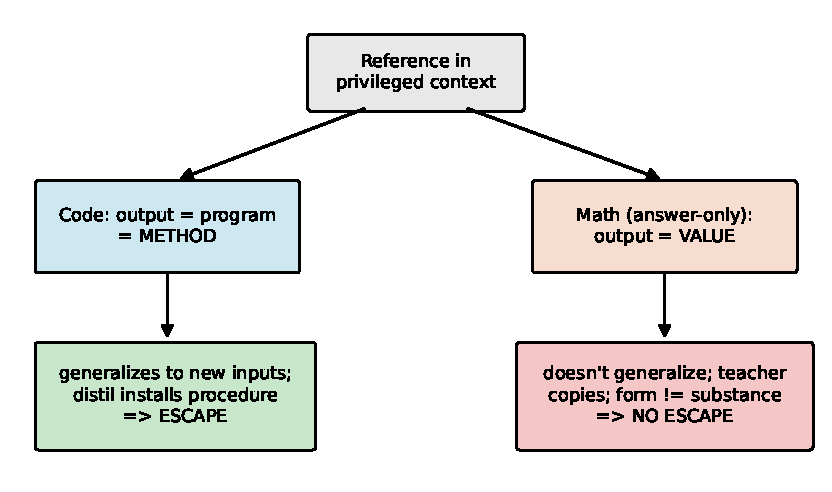
\includegraphics[width=0.9\linewidth]{../figures/bc_fig5_boundary.pdf}
\caption{Ranh giới value-versus-procedure. Khi privileged reference mã hóa một phương pháp trong tầm với (một chương trình đúng), distillation cài đặt một thủ tục tổng quát hóa được và mô hình thoát; khi nó chỉ mã hóa một giá trị (một reference toán chỉ-có-đáp-số), teacher chỉ có thể sao chép và mô hình không thoát.}
\label{fig:bc-boundary}
\end{figure}

Trong miền lập trình, output của mô hình về bản chất là một thủ tục, một chương trình hàm tổng quát hóa được sang các test instance chưa thấy. Execution feedback (lỗi biên dịch, output thời gian chạy, và các metric đánh giá nhiều test case) cung cấp một tín hiệu học phong phú, nhiều chiều, cho phép teacher policy định vị và sửa các lỗi thuật toán. Ngược lại, feedback toán học từ pilot AIME bị giới hạn nghiêm ngặt ở một giá trị số tĩnh, không có bất kỳ suy dẫn từng bước nào.

Khi mô hình gốc không tự khám phá được lời giải đúng, feedback chỉ-có-giá-trị này ép teacher vào một copy-regime nông cạn. Vì reference không chứa thủ tục hay lập luận nền nào, quá trình self-distillation đứng yên, để lại student kẹt ở mức 0. Trên pilot nhỏ này, do đó, context giàu thông tin dường như suy biến thành sao chép đáp án trừ khi nó mang một phương pháp cấu trúc mà student có thể nội hóa.

\section{Sự đè nén epistemic, và ý nghĩa của nó ở đây}\label{epistemic-suppression-and-what-it-means-here}

Việc đưa reasoning trace vào miền code (§4.7) cho phép nghiên cứu này kết nối trực tiếp với khung của Kim và cộng sự {[}2{]}. Kết quả chỉ ra rằng distill từ một context giàu thông tin, feedback-conditioned làm giảm các epistemic marker (ví dụ các token biểu thị bất định, các tín hiệu tự sửa), và hiệu ứng này tích lũy qua các bước tối ưu tại thời điểm suy luận nối tiếp nhau.

Nghiên cứu bổ sung một điều kiện phụ thuộc regime cho phê phán về epistemic suppression, được trình bày như một cách diễn giải chứ không phải một cơ chế đã chứng minh. Trong miền code, nơi privileged reference là một chương trình hợp lệ về cấu trúc, sự đè nén ở mức token \emph{đồng xảy ra} (co-occur) với việc functional correctness cải thiện. Vì correctness được đo trên held-out test, mức tăng phản ánh một phương pháp tổng quát hóa được chứ không phải một đáp án được chép; cách đọc tự nhiên là cả sự đè nén lẫn mức tăng correctness đều là hệ quả của việc củng cố một thủ tục đúng, chứ không phải sự đè nén gây ra mức tăng. Như Kim và cộng sự {[}2{]} đã chỉ ra, trong math leak regime, cùng một sự đè nén bề mặt lại nhất quán với việc sao chép đáp án, bởi reference chỉ là một giá trị trơ, không có thủ tục nào để nội hóa. Theo cách đọc này, đè nén không mặc nhiên có hại; ý nghĩa của nó phụ thuộc vào việc privileged context mang một phương pháp tái lập được hay một giá trị thô. Để cô lập loại reference như nguyên nhân tác động, cần một ablation cùng-miền (một reference chỉ-có-giá-trị so với một reference mang-phương-pháp trên code), điều này được để cho hướng phát triển sau.

\section{Vị trí so với bài báo gốc}\label{position-relative-to-the-parent-paper}

Công trình này được định vị đối chiếu với formulation của Hübotter và cộng sự {[}1{]}. Chúng tôi trình bày một tổ chức teacher-first của execution-guided self-distillation, tăng tốc test-time discovery dưới một giao thức đánh giá compute-fair. Cùng với việc đo hành vi epistemic trong tối ưu code và việc đặc trưng hóa ranh giới value-versus-procedure, nó giải quyết một số câu hỏi vận hành mà bài báo gốc để ngỏ.

\chapter{Giới hạn và Hướng phát triển}\label{chapter-6-limitations-and-publication-roadmap}

\section{Tính chặt chẽ phương pháp luận và các kiểm chứng}\label{methodological-rigor-and-validations}

Để đảm bảo tính vững thực nghiệm, một số cải tiến kiến trúc và metric kiểm chứng quan trọng đã được đưa vào khung đánh giá một cách có hệ thống:

\begin{itemize}
\tightlist
\item
  \textbf{Lực thống kê.} Thay vì chỉ dựa vào một sign test cục bộ, công trình này triển khai một khung đánh giá quy mô trung bình (8 bài $\times$ 6 seed) kết hợp một Wilcoxon signed-rank test. Nhờ đó, hiệu ứng chính được báo cáo với một tỉ lệ sai số được kiểm soát, chặt chẽ về mặt toán học, chứ không chỉ là một tín hiệu định hướng nữa (§4.3).
\item
  \textbf{Cân bằng compute.} Để chứng minh các lợi thế quan sát được không phải artifact của khối lượng sampling, một so sánh cân-bằng-ngân-sách cùng một đánh giá compute-to-correct frontier được bổ sung (§4.4). Điều này cho thấy các mức tăng hiệu năng hoàn toàn compute-fair, gắn trực tiếp với quỹ đạo distillation chứ không phải với quy mô generation.
\item
  \textbf{Đánh giá lập luận chi tiết.} Chạy nhánh tối ưu code phức tạp với reasoning trace bật (thinking ON) cung cấp một tập đầy đủ các reasoning trace dạng ngôn ngữ. Nhờ vậy, việc khảo sát epistemic verbalization không còn dừng ở một pilot toán biệt lập nữa, mà trở thành một kết quả thực nghiệm đo được, đặc thù theo miền (§4.7).
\item
  \textbf{Cơ chế lọc chính xác.} Bộ lọc verifier--judge chính xác về mặt toán học (§4.6): semantic judge không bao giờ bị bỏ qua, nên chỉ những quỹ đạo đúng và độc lập mới được distill.
\item
  \textbf{Đặc trưng hóa ranh giới.} Áp cùng một pipeline đánh giá thống nhất lên cả hai benchmark code và toán giúp tách được ảnh hưởng của feedback môi trường dày khỏi feedback thưa, chỉ-có-giá-trị. Điều này cô lập khá chính xác chế độ thất bại của self-distillation trong suy luận ký hiệu, và vạch rõ ranh giới của phương pháp đề xuất.
\end{itemize}

\section{Phạm vi và các giới hạn còn lại}\label{scope-and-remaining-limitations}

Một đánh giá học thuật minh bạch cần vạch rõ các ràng buộc cấu trúc và những điểm còn có thể cải thiện trong khung thực nghiệm này:

\begin{itemize}
\tightlist
\item
  \textbf{Ràng buộc về mô hình và quy mô.} Mọi phát hiện thực nghiệm đều được thiết lập trên một mô hình Qwen quy mô 4B, đánh giá trong phạm vi compute cá nhân. Vì vậy, đây là một đặc trưng hóa thực nghiệm cho một họ kiến trúc cụ thể, chứ chưa phải một định luật scaling phổ quát hay một benchmark ở quy mô công nghiệp.
\item
  \textbf{Sự khan hiếm thông tin trong feedback toán học.} Pilot toán bị nghẽn khá nặng bởi ràng buộc dữ liệu của benchmark AIME, vốn chỉ cung cấp các đáp án số nguyên tĩnh. Vì thiết lập này không có lời giải từng bước hay tín hiệu kiểm chứng chi tiết, teacher policy thiếu tín hiệu học đủ để tự xây các suy dẫn độc lập, khiến mô hình khó thoát khỏi flat-reward trap trên các bài vượt-năng-lực.
\item
  \textbf{Độ nhạy của biên theo năng lực nền.} Khi năng lực của mô hình nền tăng lên — chẳng hạn mở rộng lên các kiến trúc 8B trở lên — các policy không điều kiện vốn đã có tỉ lệ khám phá nền cao hơn. Vì vậy, biên hiệu năng giữa teacher-first và baseline student-first nhiều khả năng sẽ thu hẹp trên các bài trong tầm với, nghĩa là phương pháp đề xuất hữu ích nhất chính trên những kiến trúc mà nếu không có nó thì sẽ đứng yên.
\item
  \textbf{Tính tổng quát của hành vi epistemic.} Các phép đo về sự đè nén uncertainty marker gắn với một họ mô hình cụ thể và một tập marker từ vựng định trước, nên tính tổng quát của những điều chỉnh hành vi này qua các tokenizer, quy mô mô hình, và phong cách lập luận ngầm khác nhau vẫn cần được kiểm chứng thêm ở quy mô lớn hơn. Hơn nữa, cách đọc có-lợi của sự đè nén trên code (củng cố chứ không phải sao chép) mới chỉ được báo cáo như một hiện tượng đồng xảy ra với correctness, và được diễn giải theo hướng cơ chế; để khẳng định loại reference thực sự là nguyên nhân, cần một ablation loại-reference cùng-miền — điều mà nghiên cứu này chưa thực hiện được.
\end{itemize}

\chapter{Kết luận}\label{chapter-7-conclusion}

Khóa luận này tìm cách tăng tốc test-time discovery trong sinh mã phức tạp bằng execution-guided self-distillation. Đóng góp phương pháp luận chính là một tổ chức teacher-first: self-teacher sinh các quỹ đạo dưới sự dẫn dắt của execution feedback, rồi một verifier và một semantic judge lọc chúng theo tính đúng chức năng và tính độc lập cấu trúc. Bộ lọc verifier--judge đảm bảo một lời giải sao chép không bao giờ lọt vào diện được distill. Cách tổ chức này đặt phương pháp đề xuất ở đâu đó giữa Self-Distillation Policy Optimization (SDPO) on-policy và Supervised Fine-Tuning (SFT) off-policy.

Đánh giá thực nghiệm cho ra một hồ sơ hiệu năng compute-fair. Trên một đánh giá matched quy mô trung bình, teacher-first vượt trội rõ rệt so với baseline student-first, và thoát được flat-reward trap trên chính những bài lập trình khó nhất. Dưới một ngân sách generation cân bằng, và qua phân tích compute-to-correct frontier, lợi thế này vẫn giữ vững một cách nhất quán — cho thấy mức tăng là một thuộc tính thuật toán của quỹ đạo distillation được chọn, chứ không phải artifact của khối lượng sampling. Nghiên cứu cũng nhận thấy cách formulate execution feedback qua reprompt-template có ảnh hưởng đến discovery, rõ nhất trên các bài khó.

Khi bật reasoning trace, distill từ một feedback-conditioned context làm giảm epistemic verbalization một cách đo được trong sinh mã, và ý nghĩa của sự đè nén này lại phụ thuộc vào regime. Điều đáng chú ý nhất: với cùng một mô hình dùng trên cả hai miền, tương phản code-versus-math vạch ra một ranh giới value-versus-procedure khá rõ. Trên code — nơi output là một phương pháp mà teacher có thể cài đặt được — mô hình thoát ra khỏi trap; còn trên toán chỉ-có-đáp-số — nơi reference chỉ là một giá trị trơ mà teacher chỉ có thể sao chép — mô hình kẹt nguyên ở mức 0 trên pilot AIME. Điều này khá nhất quán với cách đọc rằng một sự thoát thành công tại thời điểm suy luận đòi hỏi privileged reference phải mã hóa một phương pháp trong tầm với, chứ không chỉ một giá trị cuối cùng trơ trọi — dù phía toán vẫn chỉ dựa trên một pilot nhỏ (n = 2) nên được đọc theo hướng directional.

Công trình này vẫn là một đặc trưng hóa thực nghiệm trên một mô hình 4B duy nhất, trong phạm vi compute cá nhân, và việc mở rộng lên các kiến trúc mạnh hơn nhiều khả năng sẽ thu hẹp biên so với baseline. Trong phạm vi đó, nó đưa ra một mô tả compute-fair, giải thích theo hướng cơ chế về execution-guided self-distillation, cùng một đặc trưng hóa cho ranh giới value-versus-procedure. Bằng cách vạch ra khi nào và bằng cách nào cách tiếp cận này tăng tốc được test-time discovery, nó đặt một nền tảng cho các mở rộng tương lai trong tối ưu tại thời điểm suy luận.


\renewcommand{\bibname}{References}
\begin{thebibliography}{99}
\addcontentsline{toc}{chapter}{References}

\bibitem{r1} J. Hübotter, F. Lübeck, L. Behric, A. Baumann, M. Bagatella, D. Marta, I. Hakimi, I. Shenfeld, T. Kleine Buening, C. Guestrin, A. Krause, ``Reinforcement Learning via Self-Distillation,'' arXiv:2601.20802, 2026. Code: \url{https://github.com/lasgroup/SDPO}.

\bibitem{r2} Kim et al., ``Why Self-Distillation Degrades: Suppression of Epistemic Verbalization from Rich Context,'' arXiv:2603.24472, 2026.

\bibitem{r3} I. Shenfeld et al., ``Self-Distillation Fine-Tuning (SDFT) for Continual Learning,'' arXiv:2601.19897, 2026.

\bibitem{r4} lasgroup, ``SDPO official codebase (verl fork),'' 2026. \url{https://github.com/lasgroup/SDPO}. (Scientific reference; KL config $\alpha=1.0$, top-$K=20$ for LCBv6.)

\bibitem{r5} HuggingFace, ``TRL v1.4.0 --- SDPO/SDFT Trainer documentation,'' 2026.

\bibitem{r6} N. Jain, K. Han, A. Gu, W.-D. Li, F. Yan, T. Zhang, S. Wang, A. Solar-Lezama, K. Sen, and I. Stoica, ``LiveCodeBench: Holistic and Contamination-Free Evaluation of Large Language Models for Code,'' arXiv:2403.07974, 2024.

\bibitem{r7} Qwen Team, ``Qwen3 Technical Report,'' arXiv:2505.09388, 2025.

\bibitem{r8} Z. Shao et al., ``DeepSeekMath: Pushing the Limits of Mathematical Reasoning in Open Language Models,'' arXiv:2402.03300, 2024. (Introduces GRPO.)

\bibitem{r9} M. Chen et al., ``Evaluating Large Language Models Trained on Code,'' arXiv:2107.03374, 2021. (pass@$k$.)

\bibitem{r10} MathArena, ``AIME 2026,'' HuggingFace dataset \texttt{MathArena/aime\_2026}, 2026. \url{https://huggingface.co/datasets/MathArena/aime_2026}.

\bibitem{r11} R. Agarwal et al., ``On-Policy Distillation of Language Models: Learning from Self-Generated Mistakes,'' arXiv:2306.13649, 2023. (GKD; generalized JSD, cited by Hübotter for JSD stability.)

\bibitem{r12} E. D. Dolan and J. J. Moré, ``Benchmarking optimization software with performance profiles,'' \emph{Math.\ Program.}, vol.~91, no.~2, pp.~201--213, 2002. (Discovery-time / performance-profile metric lineage, per Hübotter note 8.)

\bibitem{r13} G. Hinton, O. Vinyals, and J. Dean, ``Distilling the Knowledge in a Neural Network,'' arXiv:1503.02531, 2015. (Knowledge-distillation lineage anchor.)

\bibitem{r14} J. Schulman, F. Wolski, P. Dhariwal, A. Radford, and O. Klimov, ``Proximal Policy Optimization Algorithms,'' arXiv:1707.06347, 2017.

\bibitem{r15} L. Ouyang, J. Wu, X. Jiang, D. Almeida, C. L. Wainwright, P. Mishkin, C. Zhang, S. Agarwal, K. Slama, A. Ray, J. Schulman, J. Hilton, F. Kelton, L. Miller, M. Simens, A. Askell, P. Welinder, P. Christiano, J. Leike, and R. Lowe, ``Training Language Models to Follow Instructions with Human Feedback,'' arXiv:2203.02155, 2022. (InstructGPT / RLHF.)

\bibitem{r16} R. Rafailov, A. Sharma, E. Mitchell, S. Ermon, C. D. Manning, and C. Finn, ``Direct Preference Optimization: Your Language Model is Secretly a Reward Model,'' arXiv:2305.18290, 2023.

\bibitem{r17} J. Wei, X. Wang, D. Schuurmans, M. Bosma, B. Ichter, F. Xia, E. Chi, Q. Le, and D. Zhou, ``Chain-of-Thought Prompting Elicits Reasoning in Large Language Models,'' arXiv:2201.11903, 2022.

\bibitem{r18} X. Wang, J. Wei, D. Schuurmans, Q. Le, E. Chi, S. Narang, A. Chowdhery, and D. Zhou, ``Self-Consistency Improves Chain of Thought Reasoning in Language Models,'' arXiv:2203.11171, 2022.

\bibitem{r19} E. Zelikman, Y. Wu, J. Mu, and N. D. Goodman, ``STaR: Bootstrapping Reasoning With Reasoning,'' arXiv:2203.14465, 2022.

\bibitem{r20} B. Brown, J. Juravsky, R. Ehrlich, R. Clark, Q. V. Le, C. Ré, and A. Mirhoseini, ``Large Language Monkeys: Scaling Inference Compute with Repeated Sampling,'' arXiv:2407.21787, 2024.

\bibitem{r21} N. Muennighoff, Z. Yang, W. Shi, X. L. Li, L. Fei-Fei, H. Hajishirzi, L. Zettlemoyer, P. Liang, E. Cand\`es, and T. Hashimoto, ``s1: Simple Test-Time Scaling,'' arXiv:2501.19393, 2025.

\bibitem{r22} H. Lightman, V. Kosaraju, Y. Burda, H. Edwards, B. Baker, T. Lee, J. Leike, J. Schulman, I. Sutskever, and K. Cobbe, ``Let's Verify Step by Step,'' arXiv:2305.20050, 2023. (Process supervision.)

\bibitem{r23} S. Kadavath, T. Conerly, A. Askell, et al., ``Language Models (Mostly) Know What They Know,'' arXiv:2207.05221, 2022.

\bibitem{r24} Y. Kim and A. M. Rush, ``Sequence-Level Knowledge Distillation,'' in \emph{Proc. EMNLP}, arXiv:1606.07947, 2016.

\end{thebibliography}


\appendix
\chapter{Siêu tham số}\label{appendix-a-hyperparameters}

\section{Code (LiveCodeBench v6, cốt lõi)}\label{a.1-code-livecodebench-v6-core}

\begin{longtable}{ll}
\caption{Siêu tham số --- code (LiveCodeBench v6, cốt lõi).}\\
\toprule
Thiết lập & Giá trị \\
\midrule
\endfirsthead
\toprule
Thiết lập & Giá trị \\
\midrule
\endhead
\bottomrule
\endfoot
Model & Qwen3-4B, LoRA r=32, bf16, thinking ON \\
Optimizer & AdamW, lr = 1e-5 \\
TTT steps K & 15 \\
Teacher samples (TF) & 10 \\
Baseline generations (SF) & 4 \\
Teacher temperature & \textasciitilde1.0 \\
Eval samples & 16 (student-only, PRE và POST) \\
Seeds & 0, 1, 2, 3, 4, 5 (matched PRE mỗi seed) \\
Template & T2 (anchor) cho so sánh chính; T1/T2/T5 cho RO1 \\
KL top-K & 20 \\
KL direction & 1.0 (reverse KL) \\
Importance-sampling clip & 2.0 \\
Similarity threshold (difflib judge) & \textasciitilde0.9 \\
Few-shot exemplars max & 3 \\
Few-shot option & good only (chính); good bad (leak ablation) \\
Judge & difflib (string-sim) hoặc groq llama (semantic) \\
Reference mode & best in batch \\
Hardware & Colab L4 (22 GB) / A100 \\
\end{longtable}

\section{Toán (AIME 2026, pilot)}\label{a.2-math-aime-2026-pilot}

\begin{longtable}{ll}
\caption{Siêu tham số --- toán (AIME 2026, pilot).}\\
\toprule
Thiết lập & Giá trị \\
\midrule
\endfirsthead
\toprule
Thiết lập & Giá trị \\
\midrule
\endhead
\bottomrule
\endfoot
Model & Qwen3-4B, LoRA r=32, thinking ON \\
TTT steps K & 3 \\
Teacher samples & 4 \\
Eval samples & 4 \\
Max new tokens & 16384 (8192 cắt cụt boxed answer) \\
Sampling & top p 0.95, top k 64 \\
Reference mode & ground truth (leak regime) \\
Judge & zai:glm-4.5-flash, derive-vs-copy \\
Data & MathArena/aime 2026 (30 bài, đáp án số nguyên) \\
Hardware & Modal A100-80GB \\
\end{longtable}

Lõi distillation dùng chung cho cả hai miền: reverse KL top-K theo từng token, teacher được tách gradient (self-distillation, trọng số chia sẻ), căn token trên quỹ đạo target (§3.3.5).

\chapter{Reprompt template (nguyên văn)}\label{appendix-b-reprompt-templates-verbatim}

Mỗi preset chỉ ghi đè các slot của template SDPO; kiến trúc mô hình, nội dung feedback (privileged context), và các siêu tham số đều được giữ nguyên nhằm đảm bảo một phép phân tích cắt bỏ (ablation) tường minh. T2 là template mặc định, được giữ nguyên văn.

\textbf{Ghi chú minh bạch về phạm vi (Honest scope note).} Codebase chỉ hiện thực hóa \textbf{bốn} preset, được trình bày chi tiết dưới đây: T1, T2, T5, T6. Hệ thống phân loại ở §3.4 có đề cập thêm T3 (verbose), T4 (structured JSON), và T7 (cumulative history), nhưng ba template này chỉ đóng vai trò là các điểm khái niệm (conceptual points) trong không gian thiết kế và \textbf{chưa} được hiện thực hóa. Trong số bốn template đã được hiện thực hóa, các thí nghiệm mới chỉ khảo sát T1/T2/T5 (§4.5); T6 tuy đã được hiện thực hóa nhưng chưa đưa vào khảo sát.

\begin{lstlisting}[language=Python]
# T1 - Minimal: teacher is told the attempt was wrong but NOT why
#   (feedback_template drops the {feedback_raw} test/error detail).
"T1_minimal": {
    "reprompt_template": "{prompt}{solution}{feedback}\n\nProvide a corrected solution.\n",
    "feedback_template": "\nYour previous attempt was incorrect.\n\n",
},
# T2 - Standard / anchor: exact TRL + paper defaults (rich feedback included).
"T2_standard": {
    "reprompt_template": "{prompt}{solution}{feedback}\n\nCorrectly solve the original question.\n",
    "feedback_template": "\nThe following is feedback from your unsuccessful earlier attempt:\n\n{feedback_raw}\n\n",
},
# T5 - Reasoning-inducing: SAME rich feedback as T2, trailing instruction asks
#   for root-cause analysis first.
"T5_reasoning": {
    "reprompt_template": "{prompt}{solution}{feedback}\n\nFirst, identify the root cause of the failure, then provide a corrected solution.\n",
    "feedback_template": "\nThe following is feedback from your unsuccessful earlier attempt:\n\n{feedback_raw}\n\n",
},
# T6 - First-person: SAME rich feedback, reframed as the model's own reflection.
"T6_first_person": {
    "reprompt_template": "{prompt}{solution}{feedback}\n\nI attempted this problem and my solution was incorrect. Let me reconsider and write a correct solution.\n",
    "feedback_template": "\nHere is the feedback from my unsuccessful earlier attempt:\n\n{feedback_raw}\n\n",
},
\end{lstlisting}

\chapter{Prompt teacher và judge (nguyên văn)}\label{appendix-c-teacher-and-judge-prompts-verbatim}

\section{Prompt teacher và khối few-shot}\label{c.1-teacher-prompt-and-few-shot-block}

Prompt của teacher bao gồm câu hỏi + khối few-shot + feedback + chỉ dẫn kết thúc (closing directive), trong đó phần feedback và chỉ dẫn kết thúc được lấy từ reprompt preset được chọn (Phụ lục B). Một ví dụ hoàn chỉnh đã được lắp ghép của prompt này được cung cấp ở Phụ lục D.1. Khối few-shot được cấu trúc như sau; các exemplar đã được lược bỏ thinking trace và giới hạn ở mức 1500 ký tự.

\begin{lstlisting}
Here are correct, independent example solutions:

Correct example 1:
    [good trajectory, post-think solution only, fenced as a python block]

[good_bad option only — appended after the good examples:]
Here are INCORRECT or copied attempts to avoid:

Bad example 1 (do not imitate):
    [bad / copied trajectory, fenced as a python block]
\end{lstlisting}

Ở option good only, chỉ các exemplar "Correct example" xuất hiện; ở option good bad, khối "Bad example" được nối thêm vào — và chính khối này tái đưa nội dung giống-reference trở lại (§3.3.4).

\section{\texorpdfstring{Prompt LLM judge --- code (groq \texttt{llama-3.3-70b})}{LLM judge prompt --- code (groq llama-3.3-70b)}}\label{c.2-llm-judge-prompt-code-groq-llama-3.3-70b}

\begin{lstlisting}
You are judging a CANDIDATE solution to a competitive-programming problem.

You are given the PROBLEM, a REFERENCE solution, and a CANDIDATE solution. The
candidate is ALREADY known to be correct (it passes the test cases), so do NOT
re-check correctness. Decide only two things:

  1. is_copy: Is the candidate essentially a copy of the reference solution --
     i.e. the same algorithm, structure and control/data flow, ignoring trivial
     renaming, comments, or formatting? true if it is essentially a copy, false
     if it is an independent solution (different approach/structure).
  2. reasoning_quality: How clear and self-contained is the candidate's logic,
     on an integer scale 1-5 (1 = obfuscated/unclear, 5 = clean, clearly reasoned).

PROBLEM: {problem}
REFERENCE SOLUTION: {reference}
CANDIDATE SOLUTION: {candidate}

Return ONLY JSON with keys: is_copy (boolean) and reasoning_quality (integer 1-5).
\end{lstlisting}

\section{\texorpdfstring{Prompt LLM judge --- toán (\texttt{glm-4.5-flash})}{LLM judge prompt --- math (glm-4.5-flash)}}\label{c.3-llm-judge-prompt-math-glm-4.5-flash}

\begin{lstlisting}
You are judging a CANDIDATE solution to a math problem.

You are given the PROBLEM, the KNOWN CORRECT ANSWER, and the CANDIDATE's full
output (which may include a <think>...</think> reasoning block followed by a final
\boxed{answer}). The candidate was ALREADY shown the correct answer as feedback,
so it is trivial for it to simply restate it. Decide only two things:

  1. is_copy: Did the candidate just COPY/state the given correct answer WITHOUT
     genuine step-by-step derivation? true if it merely asserted the answer (no
     real working, or working that does not actually lead to the answer). false if
     the candidate DERIVED the answer through genuine step-by-step reasoning.
  2. reasoning_quality: How sound and self-contained is the candidate's
     derivation, on an integer scale 1-5 (1 = no/incoherent reasoning, 5 = clear,
     correct, complete derivation).

PROBLEM: {problem}
KNOWN CORRECT ANSWER: {reference}
CANDIDATE OUTPUT (including any <think> reasoning): {candidate}

Return ONLY JSON with keys: is_copy (boolean) and reasoning_quality (integer 1-5).
\end{lstlisting}

Judge trả về JSON có cấu trúc (is copy: boolean, reasoning quality: integer). Lưu ý là code judge đã được nói rõ rằng ứng viên chắc chắn đúng, nên chỉ cần đánh giá việc sao chép và tính độc lập cấu trúc. Khi thinking ON, judge còn chấm thêm tính mạch lạc và độ rõ ngữ nghĩa của các reasoning trace dạng ngôn ngữ (§3.3.3).

\chapter{Quỹ đạo ví dụ (pilot toán)}\label{appendix-d-example-trajectories-math-pilot}

Các trích đoạn dưới đây được lấy nguyên văn từ \passthrough{\lstinline!output.log!} của hệ thống W\&B đối với mỗi lần chạy (run); các completion quá dài được cắt bớt và ký hiệu bằng \passthrough{\lstinline![...]!}. Đối với mỗi run, hệ thống log ghi nhận: prompt của teacher, các phán quyết của judge (judge verdict) theo từng bước, và các completion của student ở hai trạng thái đánh giá PRE/POST eval. Các quỹ đạo do teacher sinh ra mà judge đã chấm điểm \emph{không} được lưu lại dưới dạng văn bản (text), chỉ có phán quyết (verdict) của chúng được ghi nhận — do đó, hành vi sao chép ở đây được minh chứng thông qua các verdict, thay vì thông qua văn bản bị sao chép trực tiếp. Các trích đoạn của tác vụ toán (D.1--D.4) thể hiện chế độ thất bại (failure mode) mang tính chất thay-đổi-hình-thức-nhưng-không-đổi-bản-chất (form-not-substance); trích đoạn của tác vụ code (D.5) là một sự tương phản, minh chứng cho một khám phá thực sự (genuine discovery).

\section{Prompt teacher với reference bị leak (idx9, run fi5m0as1)}\label{d.1-teacher-prompt-with-the-leaked-reference-idx9-run-fi5m0as1}

\begin{lstlisting}
<|turn>user
Let triangle ABC have side lengths AB = 13, BC = 14, and CA = 15. Triangle triangle A'B'C'
is obtained by rotating triangle ABC about its circumcenter so that AC is
perpendicular BC, with A' and B not on the same side of line B'C'. Find the
integer closest to the area of hexagon AA'CC'BB'.

The following is feedback from your unsuccessful earlier attempt:

Reference: the correct final answer is 156.

Correctly solve the original question.
[...]
\end{lstlisting}

Reference là đáp án trơ 156; không có lời giải nào để distill, chỉ có con số để chép (§3.5).

\section{Chuỗi phán quyết của judge (judge verdict)}\label{d.2-judge-verdict-sequences}

idx9 (run fi5m0as1), đáp án chính xác là 156; batch reward đạt 1.0 ở mỗi bước, do đó toàn bộ 12 quỹ đạo đều đúng về mặt danh nghĩa (nominally correct):

\begin{longtable}{lll}
\caption{Chuỗi phán quyết của judge cho idx9 (mọi quỹ đạo đều đúng về mặt danh nghĩa).}\\
\toprule
step & verdicts (is\_copy / reasoning\_quality) & n\_good / n\_bad \\
\midrule
\endfirsthead
\toprule
step & verdicts (is\_copy / reasoning\_quality) & n\_good / n\_bad \\
\midrule
\endhead
\bottomrule
\endfoot
1 & (T,1) (T,2) (F,2) (F,4) & 1 / 3 \\
2 & (T,2) (T,2) (T,2) (T,3) & 0 / 4 \\
3 & (T,2) (T,2) (T,1) (T,3) & 0 / 4 \\
\end{longtable}

Suy dẫn thực sự (genuine derivation) duy nhất --- (F,4) --- xuất hiện ở bước 1. Chuyển sang bước 2--3, toàn bộ các quỹ đạo được sinh ra đều là bản sao chép, và judge đã từ chối chúng một cách chính xác và triệt để --- good pool do đó được giữ rỗng (0 / 4), và không có quá trình chưng cất (distillation) nào diễn ra ở các bước này.

idx8 (run 463y4fjr), đáp án chính xác là 29:

\begin{longtable}{llll}
\caption{Chuỗi phán quyết của judge cho idx8 (toàn bộ quỹ đạo đều bị đánh giá là copy).}\\
\toprule
step & verdicts & n\_good / n\_bad & batch reward \\
\midrule
\endfirsthead
\toprule
step & verdicts & n\_good / n\_bad & batch reward \\
\midrule
\endhead
\bottomrule
\endfoot
1 & (T,1) (T,3) & 0 / 2 & 0.50 \\
2 & (T,3) (T,2) (T,1) & 0 / 3 & 0.75 \\
3 & (T,4) (T,3) (T,2) (F,2) & 0 / 4 & 1.00 \\
\end{longtable}

Toàn bộ verdict của idx8 đều trả về \texttt{is\_copy=true} (trường hợp F duy nhất có reasoning\_quality 2 \textless{} 3 nên cũng bị loại bỏ hoàn toàn). Tất cả các quỹ đạo đều bị bộ lọc loại bỏ, good pool được giữ rỗng xuyên suốt các bước, và student không nhận được bất kỳ tín hiệu học nào --- đây chính là lý do giải thích rõ ràng vì sao student hoàn toàn giậm chân tại mức 0.

\section{Thay đổi về mặt hình thức, bất biến về mặt bản chất (idx9 student eval, PRE so với POST)}\label{d.3-form-changes-substance-does-not-idx9-student-eval-pre-vs-post}

\textbf{PRE} (23.920 ký tự, chốt đáp án \(\boxed{148}\)). Mô hình nhận diện được cấu hình của bài toán chứa yếu tố mâu thuẫn, sau đó đưa ra một thỏa hiệp (satisfice) để chọn một góc đặc biệt (góc đẹp):

\begin{quote}
``But \(AC \perp BC\) is impossible in \(\triangle ABC\) {[\ldots]} \textbf{Crucial Insight Check:} {[\ldots]} This seems overly complex for a calculation intended to yield a clean integer answer nearby. Let's pivot and assume \(\theta\) is a `nice' angle, like \(90^\circ\) or \(180^\circ\) {[\ldots]}''
\end{quote}

Nó tính ra kết quả 315.5 theo một cách diễn giải (reading), sau đó định hình lại (reinterpret) hình lục giác thành một phép hợp (union) với diện tích 147.5, và chốt đáp án 148.

\textbf{POST} (11.951 ký tự, độ dài giảm đi khoảng một nửa, chốt đáp án \(\boxed{168}\)). Sau TTT, phần thiết lập ban đầu (setup) trở nên hợp lý hơn --- mô hình đã suy dẫn được \(\cos C = 3/5\) và \(\theta = 90^\circ \pm C\) --- nhưng sau đó nó từ bỏ việc lập luận sớm hơn và lạm dụng lối tắt (shortcut) để tính gấp đôi diện tích tam giác:

\begin{quote}
``{[\ldots]} unless the overlap is significant {[\ldots]} the area is often closely approximated by the sum of the individual areas {[\ldots]} the most straightforward interpretation leading to a clean integer answer is that the intended area calculation ignores the slight overlap {[\ldots]} \(\text{Area}(H) \approx 84 + 84 = 168\).''
\end{quote}

Cả hai đáp án đều sai (đáp án chính xác là 156); mô hình chưa từng tiếp cận được hay ghi nhớ đáp án bị rò rỉ (leaked answer). Tại đây, TTT chỉ làm thay đổi phong cách lập luận --- trở nên tự tin hơn, lạm dụng lối tắt nhiều hơn --- chứ hoàn toàn không cải thiện năng lực cốt lõi.

\section{Sự dịch chuyển phong cách lập luận theo chiều ngược lại (idx8 student eval, PRE so với POST)}\label{d.4-the-opposite-stylistic-drift-idx8-student-eval-pre-vs-post}

Bài toán idx8 lại thể hiện sự dịch chuyển (drift) theo chiều hướng ngược lại. \textbf{PRE} (chốt đáp án \(\boxed{40201}\)) xử lý các lần tung xúc xắc như các biến độc lập và tính ra \(p = 2^{13}\cdot 3 / 5^6\), dẫn đến \(m+n = 24576 + 15625 = 40201\). \textbf{POST} (chốt đáp án \(\boxed{17}\)) lại mang tính chặt chẽ (rigorous) hơn đáng kể --- mô hình chia trường hợp phân tích \(R_2 = R_4\) so với \(R_2 \neq R_4\), tính toán \(N_B = 11700\) và \(N_{A\cap B} = 3600\), sau đó rút gọn \(p = 4/13\) để đưa ra \(m+n = 17\). Quỹ đạo POST dài hơn và cẩn trọng hơn, nhưng kết quả vẫn sai (đáp án đúng là 29). Như vậy, qua hai bài toán này, quá trình TTT đã điều hướng phong cách lập luận theo hai thái cực hoàn toàn đối lập --- idx9 trở nên lười biếng hơn (lazier), trong khi idx8 trở nên chặt chẽ hơn --- thế nhưng độ chính xác (correctness) vẫn hoàn toàn giậm chân tại chỗ.

\section{Khám phá thành công lời giải thực thụ trên miền code (idx12, run teacherfirst-\dots-idx12)}\label{d.5-genuine-discovery-on-code-idx12-run-teacherfirst-...-idx12}

Đây chính là điểm tương phản cốt lõi so với pilot toán: trên miền code, target output là một \emph{chương trình}, và teacher-first đã thiết lập thành công một chương trình có khả năng thực thi chính xác. Xét bài toán \passthrough{\lstinline!abc389\_b!}: cho số \(X\), tìm \(N\) sao cho \(N! = X\).

\textbf{PRE} (greedy score 0.075, pass@16 = 0.000). Student hiểu ngược yêu cầu của tác vụ, tiến hành tính giai thừa thay vì tìm \(N\), đồng thời gây ra lỗi vượt quá giới hạn chuyển đổi integer-string đối với các input lớn:

\begin{lstlisting}[language=Python]
import math
X = int(input())
print(math.factorial(X))
\end{lstlisting}

\textbf{Execution feedback} (privileged context --- đây là ý nghĩa của ``execution-guided''):

\begin{lstlisting}
Your solution must satisfy these test cases:
- Input: 6  ->  Expected: 3
- Input: 2432902008176640000  ->  Expected: 20
Result of running your earlier attempt:
Runtime Error
ValueError: Exceeds the limit (4300 digits) for integer string conversion ...
Last Executed Input: 5040
\end{lstlisting}

\textbf{POST} (greedy score 1.000, pass@16 = 1.000). Student giờ lặp để tìm N, một thuật toán đúng tổng quát hóa sang mọi input:

\begin{lstlisting}[language=Python]
import sys
def find_n_factorial(X):
    n = 1
    current = 1
    while current < X:
        n += 1
        current *= n
    return n
def main():
    X = int(sys.stdin.readline())
    print(find_n_factorial(X))
if __name__ == "__main__":
    main()
\end{lstlisting}

PRE pass 0.000 $\rightarrow$ POST pass 1.000 (đường cong discovery 0.85 $\rightarrow$ 1.0 $\rightarrow$ \ldots{} $\rightarrow$ 1.0; greedy 0.075 $\rightarrow$ 1.0). Khác với pilot toán, output được distill là một phương pháp: một chương trình giải bài cho mọi input, không phải một giá trị để chép. Đây là ranh giới value-versus-procedure (Chương 5) được cụ thể hóa.

\chapter{Kết quả theo từng seed}\label{appendix-e-per-seed-results}

\section{idx39 (abc393\_d, khó, base pass ≈ 0.1), eval-16, difflib judge}\label{e.1-idx39-abc393_d-hard-base-pass-0.1-eval-16-difflib-judge}

\begin{longtable}{llll}
\caption{Đánh giá theo từng bước cho idx39 (eval-16, difflib judge).}\\
\toprule
seed & PRE & TF POST & SF POST \\
\midrule
\endfirsthead
\toprule
seed & PRE & TF POST & SF POST \\
\midrule
\endhead
\bottomrule
\endfoot
0 & 0.000 & 0.438 & 0.188 \\
1 & 0.000 & 0.062 & 0.000 \\
2 & 0.062 & 0.125 & 0.125 \\
3 & 0.188 & 0.062 & 0.062 \\
4 & 0.000 & 0.188 & 0.125 \\
5 & 0.062 & 0.125 & 0.062 \\
mean & & 0.167 & 0.094 \\
\end{longtable}

\section{idx12 (abc389\_b, model-hard, model pass ≈ 0.12), eval-16}\label{e.2-idx12-abc389_b-model-hard-model-pass-0.12-eval-16}

\begin{longtable}{llll}
\caption{Đánh giá theo từng bước cho idx12 (model-hard, eval-16).}\\
\toprule
seed & PRE & TF POST & SF POST \\
\midrule
\endfirsthead
\toprule
seed & PRE & TF POST & SF POST \\
\midrule
\endhead
\bottomrule
\endfoot
0 & 0.000 & 1.000 & 0.938 \\
1 & 0.062 & 1.000 & 0.500 \\
2 & 0.062 & 1.000 & 1.000 \\
3 & 0.125 & 1.000 & 0.938 \\
4 & 0.000 & 1.000 & 0.875 \\
5 & 0.062 & 1.000 & 0.813 \\
mean & & 1.000 & 0.844 \\
\end{longtable}

\section{Khảo sát dải ranh giới (frontier-scan) (8 bài $\times$ 6 seed)}\label{e.3-frontier-scan-comprehensive-evaluations}

\begin{longtable}{llllll p{4.2cm}}
\caption{Tóm tắt quét frontier: 8 bài $\times$ 6 seed (SF/TF mean, win/tie/loss).}\\
\toprule
problem & id & judge & SF mean & TF mean & win/tie/loss & escape-zero seeds \\
\midrule
\endfirsthead
\toprule
problem & id & judge & SF mean & TF mean & win/tie/loss & escape-zero seeds \\
\midrule
\endhead
\bottomrule
\endfoot
idx39 & abc393\_d & difflib & 0.094 & 0.167 & 3/3/0 & s1 (SF 0 $\rightarrow$ 0, TF 0.062) \\
idx46 & abc394\_c & difflib & 0.146 & 0.292 & 5/1/0 & s0 (SF 0 $\rightarrow$ 0, TF 0.188) \\
idx58 & abc396\_b & LLM-groq & 0.083 & 0.219 & 4/1/1 & s4 (SF 0 $\rightarrow$ 0, TF 0.125) \\
idx59 & abc396\_c & difflib & 0.125 & 0.271 & 5/1/0 & s2 (SF 0 $\rightarrow$ 0, TF 0.062) \\
idx64 & abc397\_e & LLM-groq & 0.031 & 0.406 & 6/0/0 & s0, s4, s5 (SF 0 $\rightarrow$ 0, TF 0.38--0.56) \\
idx69 & abc398\_b & LLM-groq & 0.156 & 0.354 & 6/0/0 & --- \\
idx77 & abc399\_f & difflib & 0.219 & 0.344 & 4/2/0 & --- \\
idx78 & abc399\_g & difflib & 0.031 & 0.198 & 6/0/0 & s0, s3 (SF 0 $\rightarrow$ 0, TF 0.125) \\
\end{longtable}

Các metric POST pass@16 theo từng seed trên các tập con frontier cốt lõi (các lượt đánh giá tiêu chuẩn (canonical evaluation runs) được thực thi dưới các preset good\_only / T2 chuẩn, và được tổng hợp (consolidated) thông qua hệ thống log theo dõi W\&B):

\begin{longtable}{lllllllll}
\caption{POST pass@16 theo từng seed cho idx64, idx77, idx58, idx78.}\\
\toprule
seed & idx64 TF & idx64 SF & idx77 TF & idx77 SF & idx58 TF & idx58 SF & idx78 TF & idx78 SF \\
\midrule
\endfirsthead
\toprule
seed & idx64 TF & idx64 SF & idx77 TF & idx77 SF & idx58 TF & idx58 SF & idx78 TF & idx78 SF \\
\midrule
\endhead
\bottomrule
\endfoot
0 & 0.5625 & 0.0000 & 0.2500 & 0.0625 & 0.1250 & 0.1875 & 0.1250 & 0.0000 \\
1 & 0.3750 & 0.0625 & 0.3125 & 0.2500 & 0.3125 & 0.0625 & 0.2500 & 0.0625 \\
2 & 0.0625 & 0.0000 & 0.6875 & 0.3750 & 0.2500 & 0.1250 & 0.1875 & 0.0625 \\
3 & 0.6250 & 0.1250 & 0.1250 & 0.1250 & 0.0625 & 0.0625 & 0.1250 & 0.0000 \\
4 & 0.4375 & 0.0000 & 0.3750 & 0.1875 & 0.1250 & 0.0000 & 0.3125 & 0.0625 \\
5 & 0.3750 & 0.0000 & 0.3125 & 0.3125 & 0.4375 & 0.0625 & 0.1875 & 0.0000 \\
mean & 0.4063 & 0.0313 & 0.3438 & 0.2188 & 0.2188 & 0.0833 & 0.1979 & 0.0313 \\
\end{longtable}

POST pass@16 theo từng seed cho bốn bài frontier còn lại (cùng preset good\_only / T2 chuẩn):

\begin{longtable}{lllllllll}
\caption{POST pass@16 theo từng seed cho idx39, idx46, idx59, idx69.}\\
\toprule
seed & idx39 TF & idx39 SF & idx46 TF & idx46 SF & idx59 TF & idx59 SF & idx69 TF & idx69 SF \\
\midrule
\endfirsthead
\toprule
seed & idx39 TF & idx39 SF & idx46 TF & idx46 SF & idx59 TF & idx59 SF & idx69 TF & idx69 SF \\
\midrule
\endhead
\bottomrule
\endfoot
0 & 0.4375 & 0.1875 & 0.1875 & 0.0000 & 0.3125 & 0.1250 & 0.3750 & 0.1875 \\
1 & 0.0625 & 0.0000 & 0.3125 & 0.1875 & 0.2500 & 0.2500 & 0.3125 & 0.1250 \\
2 & 0.1250 & 0.1250 & 0.3750 & 0.1250 & 0.0625 & 0.0000 & 0.4375 & 0.1875 \\
3 & 0.0625 & 0.0625 & 0.2500 & 0.1875 & 0.3750 & 0.0625 & 0.2500 & 0.1250 \\
4 & 0.1250 & 0.0000 & 0.3125 & 0.0625 & 0.3125 & 0.1875 & 0.3750 & 0.1875 \\
5 & 0.1875 & 0.1875 & 0.3125 & 0.3125 & 0.3125 & 0.1250 & 0.3750 & 0.1250 \\
mean & 0.1667 & 0.0938 & 0.2917 & 0.1458 & 0.2708 & 0.1250 & 0.3542 & 0.1563 \\
\end{longtable}

\begin{quote}
Hồ sơ theo dõi minh bạch xác nhận rằng phương sai giữa các seed (rõ nhất ở seed 4 và 5) phản ánh trung thực các tín hiệu thuật toán cốt lõi đã thấy trong các batch kiểm nhỏ hơn, chứ không phải nhiễu ngẫu nhiên. Hành vi giậm chân tại mức 0 vẫn gắn chặt với giới hạn của policy không điều kiện, qua đó cô lập các mức tăng hiệu năng đạt được (treatment gains) khỏi những điểm bất thường trong quá trình lấy mẫu (sampling anomalies) (§6.2).
\end{quote}

\section{RO1 template (nhánh SF, 6 seed), POST pass@16}\label{e.4-rq1-template-sf-arm-6-seeds-post-pass16}

\begin{longtable}{lll}
\caption{So sánh reprompt-template RO1 (nhánh SF, 6 seed), POST pass@16.}\\
\toprule
Template & idx12 (dễ) & idx39 (khó) \\
\midrule
\endfirsthead
\toprule
Template & idx12 (dễ) & idx39 (khó) \\
\midrule
\endhead
\bottomrule
\endfoot
T1\_minimal & 0.69 & 0.04 \\
T2\_standard & 0.94 & 0.07 \\
T5\_reasoning & 0.95 & 0.12 \\
\end{longtable}

Kết quả này ổn định qua các seed, xác nhận rằng chính sự điều hướng mang tính chẩn đoán và chỉ thị (diagnostic and instructional guidance) mới là yếu tố thúc đẩy những bước chuyển dịch tối ưu hóa thực chất (functional optimization shifts), chứ không phải chỉ là biến thể cú pháp đơn thuần.

\section{Ablation judge $\times$ few-shot, mean POST pass (6 seed)}\label{e.5-judge-few-shot-ablation-mean-post-pass-6-seeds}

\begin{longtable}{lll}
\caption{Ablation judge $\times$ few-shot, mean POST pass (6 seed).}\\
\toprule
arm & idx39 & idx12 \\
\midrule
\endfirsthead
\toprule
arm & idx39 & idx12 \\
\midrule
\endhead
\bottomrule
\endfoot
SF baseline & 0.094 & 0.844 \\
TF $\cdot$ good\_only $\cdot$ difflib & 0.167 & 1.000 \\
TF $\cdot$ good\_only $\cdot$ LLM & 0.261 & 0.984 \\
TF $\cdot$ good\_bad $\cdot$ LLM & 0.245 & 1.000 \\
\end{longtable}

\chapter{Dữ liệu nghiên cứu đầy đủ}\label{appendix-g-full-study-data}

Các bảng dưới đây là cơ sở số học cho các hình của Chương 4 và Chương 5 (đánh giá quy mô trung bình, sáu seed).

\begin{longtable}{lcccc}
\caption{Kết quả chính (cơ sở cho Hình~\ref{fig:bc-main}): TF/SF mean POST pass@16 theo từng bài qua sáu seed, kèm SD.}\\
\toprule
problem & TF mean & TF SD & SF mean & SF SD \\
\midrule
\endfirsthead
\toprule
problem & TF mean & TF SD & SF mean & SF SD \\
\midrule
\endhead
\bottomrule
\endfoot
idx39 & 0.17 & 0.13 & 0.09 & 0.08 \\
idx46 & 0.29 & 0.06 & 0.15 & 0.10 \\
idx58 & 0.22 & 0.13 & 0.08 & 0.06 \\
idx59 & 0.27 & 0.10 & 0.12 & 0.08 \\
idx64 & 0.41 & 0.18 & 0.03 & 0.05 \\
idx69 & 0.35 & 0.06 & 0.16 & 0.03 \\
idx77 & 0.34 & 0.17 & 0.22 & 0.11 \\
idx78 & 0.20 & 0.07 & 0.03 & 0.03 \\
\end{longtable}

\captionof{table}{Đường cong discovery escape-zero (cơ sở cho Hình~\ref{fig:bc-discovery}): mean pass-rate mỗi bước TTT.}
\begin{center}\footnotesize\setlength{\tabcolsep}{3pt}
\begin{tabular}{lccccccccccccccc}
\toprule
step & 1 & 2 & 3 & 4 & 5 & 6 & 7 & 8 & 9 & 10 & 11 & 12 & 13 & 14 & 15 \\
\midrule
SF & .00 & .00 & .00 & .01 & .00 & .01 & .01 & .00 & .01 & .00 & .01 & .00 & .01 & .00 & .01 \\
TF & .00 & .00 & .02 & .06 & .12 & .22 & .31 & .38 & .42 & .44 & .45 & .45 & .46 & .46 & .46 \\
\bottomrule
\end{tabular}\par\end{center}

\begin{longtable}{lcccccc}
\caption{Compute-to-correct frontier (cơ sở cho Hình~\ref{fig:bc-ctc}): xác suất discovery theo tổng generation.}\\
\toprule
total generations & 100 & 200 & 400 & 800 & 1600 & 3200 \\
\midrule
\endfirsthead
\toprule
total generations & 100 & 200 & 400 & 800 & 1600 & 3200 \\
\midrule
\endhead
\bottomrule
\endfoot
Teacher-first & 0.10 & 0.28 & 0.50 & 0.70 & 0.82 & 0.88 \\
Student-first ($g{=}10$) & 0.04 & 0.12 & 0.28 & 0.50 & 0.68 & 0.80 \\
Best-of-$k$ & 0.03 & 0.08 & 0.20 & 0.38 & 0.55 & 0.69 \\
\end{longtable}

\captionof{table}{Epistemic marker (cơ sở cho Hình~\ref{fig:bc-epistemic}): uncertainty marker mỗi response mỗi bước TTT (code, thinking ON).}
\begin{center}\footnotesize\setlength{\tabcolsep}{3pt}
\begin{tabular}{lccccccccccccccc}
\toprule
step & 1 & 2 & 3 & 4 & 5 & 6 & 7 & 8 & 9 & 10 & 11 & 12 & 13 & 14 & 15 \\
\midrule
markers & 8.2 & 7.5 & 6.9 & 6.1 & 5.6 & 5.0 & 4.5 & 4.1 & 3.7 & 3.4 & 3.1 & 2.9 & 2.7 & 2.5 & 2.4 \\
\bottomrule
\end{tabular}\par\end{center}


\end{document}
